\documentclass[11pt]{article}

    \usepackage[breakable]{tcolorbox}
    \usepackage{parskip} % Stop auto-indenting (to mimic markdown behaviour)
    
    \usepackage{iftex}
    \ifPDFTeX
    	\usepackage[T1]{fontenc}
    	\usepackage{mathpazo}
    \else
    	\usepackage{fontspec}
    \fi

    % Basic figure setup, for now with no caption control since it's done
    % automatically by Pandoc (which extracts ![](path) syntax from Markdown).
    \usepackage{graphicx}
    % Maintain compatibility with old templates. Remove in nbconvert 6.0
    \let\Oldincludegraphics\includegraphics
    % Ensure that by default, figures have no caption (until we provide a
    % proper Figure object with a Caption API and a way to capture that
    % in the conversion process - todo).
    \usepackage{caption}
    \DeclareCaptionFormat{nocaption}{}
    \captionsetup{format=nocaption,aboveskip=0pt,belowskip=0pt}

    \usepackage{float}
    \floatplacement{figure}{H} % forces figures to be placed at the correct location
    \usepackage{xcolor} % Allow colors to be defined
    \usepackage{enumerate} % Needed for markdown enumerations to work
    \usepackage{geometry} % Used to adjust the document margins
    \usepackage{amsmath} % Equations
    \usepackage{amssymb} % Equations
    \usepackage{textcomp} % defines textquotesingle
    % Hack from http://tex.stackexchange.com/a/47451/13684:
    \AtBeginDocument{%
        \def\PYZsq{\textquotesingle}% Upright quotes in Pygmentized code
    }
    \usepackage{upquote} % Upright quotes for verbatim code
    \usepackage{eurosym} % defines \euro
    \usepackage[mathletters]{ucs} % Extended unicode (utf-8) support
    \usepackage{fancyvrb} % verbatim replacement that allows latex
    \usepackage{grffile} % extends the file name processing of package graphics 
                         % to support a larger range
    \makeatletter % fix for old versions of grffile with XeLaTeX
    \@ifpackagelater{grffile}{2019/11/01}
    {
      % Do nothing on new versions
    }
    {
      \def\Gread@@xetex#1{%
        \IfFileExists{"\Gin@base".bb}%
        {\Gread@eps{\Gin@base.bb}}%
        {\Gread@@xetex@aux#1}%
      }
    }
    \makeatother
    \usepackage[Export]{adjustbox} % Used to constrain images to a maximum size
    \adjustboxset{max size={0.9\linewidth}{0.9\paperheight}}

    % The hyperref package gives us a pdf with properly built
    % internal navigation ('pdf bookmarks' for the table of contents,
    % internal cross-reference links, web links for URLs, etc.)
    \usepackage{hyperref}
    % The default LaTeX title has an obnoxious amount of whitespace. By default,
    % titling removes some of it. It also provides customization options.
    \usepackage{titling}
    \usepackage{longtable} % longtable support required by pandoc >1.10
    \usepackage{booktabs}  % table support for pandoc > 1.12.2
    \usepackage[inline]{enumitem} % IRkernel/repr support (it uses the enumerate* environment)
    \usepackage[normalem]{ulem} % ulem is needed to support strikethroughs (\sout)
                                % normalem makes italics be italics, not underlines
    \usepackage{mathrsfs}
    

    
    % Colors for the hyperref package
    \definecolor{urlcolor}{rgb}{0,.145,.698}
    \definecolor{linkcolor}{rgb}{.71,0.21,0.01}
    \definecolor{citecolor}{rgb}{.12,.54,.11}

    % ANSI colors
    \definecolor{ansi-black}{HTML}{3E424D}
    \definecolor{ansi-black-intense}{HTML}{282C36}
    \definecolor{ansi-red}{HTML}{E75C58}
    \definecolor{ansi-red-intense}{HTML}{B22B31}
    \definecolor{ansi-green}{HTML}{00A250}
    \definecolor{ansi-green-intense}{HTML}{007427}
    \definecolor{ansi-yellow}{HTML}{DDB62B}
    \definecolor{ansi-yellow-intense}{HTML}{B27D12}
    \definecolor{ansi-blue}{HTML}{208FFB}
    \definecolor{ansi-blue-intense}{HTML}{0065CA}
    \definecolor{ansi-magenta}{HTML}{D160C4}
    \definecolor{ansi-magenta-intense}{HTML}{A03196}
    \definecolor{ansi-cyan}{HTML}{60C6C8}
    \definecolor{ansi-cyan-intense}{HTML}{258F8F}
    \definecolor{ansi-white}{HTML}{C5C1B4}
    \definecolor{ansi-white-intense}{HTML}{A1A6B2}
    \definecolor{ansi-default-inverse-fg}{HTML}{FFFFFF}
    \definecolor{ansi-default-inverse-bg}{HTML}{000000}

    % common color for the border for error outputs.
    \definecolor{outerrorbackground}{HTML}{FFDFDF}

    % commands and environments needed by pandoc snippets
    % extracted from the output of `pandoc -s`
    \providecommand{\tightlist}{%
      \setlength{\itemsep}{0pt}\setlength{\parskip}{0pt}}
    \DefineVerbatimEnvironment{Highlighting}{Verbatim}{commandchars=\\\{\}}
    % Add ',fontsize=\small' for more characters per line
    \newenvironment{Shaded}{}{}
    \newcommand{\KeywordTok}[1]{\textcolor[rgb]{0.00,0.44,0.13}{\textbf{{#1}}}}
    \newcommand{\DataTypeTok}[1]{\textcolor[rgb]{0.56,0.13,0.00}{{#1}}}
    \newcommand{\DecValTok}[1]{\textcolor[rgb]{0.25,0.63,0.44}{{#1}}}
    \newcommand{\BaseNTok}[1]{\textcolor[rgb]{0.25,0.63,0.44}{{#1}}}
    \newcommand{\FloatTok}[1]{\textcolor[rgb]{0.25,0.63,0.44}{{#1}}}
    \newcommand{\CharTok}[1]{\textcolor[rgb]{0.25,0.44,0.63}{{#1}}}
    \newcommand{\StringTok}[1]{\textcolor[rgb]{0.25,0.44,0.63}{{#1}}}
    \newcommand{\CommentTok}[1]{\textcolor[rgb]{0.38,0.63,0.69}{\textit{{#1}}}}
    \newcommand{\OtherTok}[1]{\textcolor[rgb]{0.00,0.44,0.13}{{#1}}}
    \newcommand{\AlertTok}[1]{\textcolor[rgb]{1.00,0.00,0.00}{\textbf{{#1}}}}
    \newcommand{\FunctionTok}[1]{\textcolor[rgb]{0.02,0.16,0.49}{{#1}}}
    \newcommand{\RegionMarkerTok}[1]{{#1}}
    \newcommand{\ErrorTok}[1]{\textcolor[rgb]{1.00,0.00,0.00}{\textbf{{#1}}}}
    \newcommand{\NormalTok}[1]{{#1}}
    
    % Additional commands for more recent versions of Pandoc
    \newcommand{\ConstantTok}[1]{\textcolor[rgb]{0.53,0.00,0.00}{{#1}}}
    \newcommand{\SpecialCharTok}[1]{\textcolor[rgb]{0.25,0.44,0.63}{{#1}}}
    \newcommand{\VerbatimStringTok}[1]{\textcolor[rgb]{0.25,0.44,0.63}{{#1}}}
    \newcommand{\SpecialStringTok}[1]{\textcolor[rgb]{0.73,0.40,0.53}{{#1}}}
    \newcommand{\ImportTok}[1]{{#1}}
    \newcommand{\DocumentationTok}[1]{\textcolor[rgb]{0.73,0.13,0.13}{\textit{{#1}}}}
    \newcommand{\AnnotationTok}[1]{\textcolor[rgb]{0.38,0.63,0.69}{\textbf{\textit{{#1}}}}}
    \newcommand{\CommentVarTok}[1]{\textcolor[rgb]{0.38,0.63,0.69}{\textbf{\textit{{#1}}}}}
    \newcommand{\VariableTok}[1]{\textcolor[rgb]{0.10,0.09,0.49}{{#1}}}
    \newcommand{\ControlFlowTok}[1]{\textcolor[rgb]{0.00,0.44,0.13}{\textbf{{#1}}}}
    \newcommand{\OperatorTok}[1]{\textcolor[rgb]{0.40,0.40,0.40}{{#1}}}
    \newcommand{\BuiltInTok}[1]{{#1}}
    \newcommand{\ExtensionTok}[1]{{#1}}
    \newcommand{\PreprocessorTok}[1]{\textcolor[rgb]{0.74,0.48,0.00}{{#1}}}
    \newcommand{\AttributeTok}[1]{\textcolor[rgb]{0.49,0.56,0.16}{{#1}}}
    \newcommand{\InformationTok}[1]{\textcolor[rgb]{0.38,0.63,0.69}{\textbf{\textit{{#1}}}}}
    \newcommand{\WarningTok}[1]{\textcolor[rgb]{0.38,0.63,0.69}{\textbf{\textit{{#1}}}}}
    
    
    % Define a nice break command that doesn't care if a line doesn't already
    % exist.
    \def\br{\hspace*{\fill} \\* }
    % Math Jax compatibility definitions
    \def\gt{>}
    \def\lt{<}
    \let\Oldtex\TeX
    \let\Oldlatex\LaTeX
    \renewcommand{\TeX}{\textrm{\Oldtex}}
    \renewcommand{\LaTeX}{\textrm{\Oldlatex}}
    % Document parameters
    % Document title
    \title{Loops}
    
    
    
    
    
% Pygments definitions
\makeatletter
\def\PY@reset{\let\PY@it=\relax \let\PY@bf=\relax%
    \let\PY@ul=\relax \let\PY@tc=\relax%
    \let\PY@bc=\relax \let\PY@ff=\relax}
\def\PY@tok#1{\csname PY@tok@#1\endcsname}
\def\PY@toks#1+{\ifx\relax#1\empty\else%
    \PY@tok{#1}\expandafter\PY@toks\fi}
\def\PY@do#1{\PY@bc{\PY@tc{\PY@ul{%
    \PY@it{\PY@bf{\PY@ff{#1}}}}}}}
\def\PY#1#2{\PY@reset\PY@toks#1+\relax+\PY@do{#2}}

\@namedef{PY@tok@w}{\def\PY@tc##1{\textcolor[rgb]{0.73,0.73,0.73}{##1}}}
\@namedef{PY@tok@c}{\let\PY@it=\textit\def\PY@tc##1{\textcolor[rgb]{0.25,0.50,0.50}{##1}}}
\@namedef{PY@tok@cp}{\def\PY@tc##1{\textcolor[rgb]{0.74,0.48,0.00}{##1}}}
\@namedef{PY@tok@k}{\let\PY@bf=\textbf\def\PY@tc##1{\textcolor[rgb]{0.00,0.50,0.00}{##1}}}
\@namedef{PY@tok@kp}{\def\PY@tc##1{\textcolor[rgb]{0.00,0.50,0.00}{##1}}}
\@namedef{PY@tok@kt}{\def\PY@tc##1{\textcolor[rgb]{0.69,0.00,0.25}{##1}}}
\@namedef{PY@tok@o}{\def\PY@tc##1{\textcolor[rgb]{0.40,0.40,0.40}{##1}}}
\@namedef{PY@tok@ow}{\let\PY@bf=\textbf\def\PY@tc##1{\textcolor[rgb]{0.67,0.13,1.00}{##1}}}
\@namedef{PY@tok@nb}{\def\PY@tc##1{\textcolor[rgb]{0.00,0.50,0.00}{##1}}}
\@namedef{PY@tok@nf}{\def\PY@tc##1{\textcolor[rgb]{0.00,0.00,1.00}{##1}}}
\@namedef{PY@tok@nc}{\let\PY@bf=\textbf\def\PY@tc##1{\textcolor[rgb]{0.00,0.00,1.00}{##1}}}
\@namedef{PY@tok@nn}{\let\PY@bf=\textbf\def\PY@tc##1{\textcolor[rgb]{0.00,0.00,1.00}{##1}}}
\@namedef{PY@tok@ne}{\let\PY@bf=\textbf\def\PY@tc##1{\textcolor[rgb]{0.82,0.25,0.23}{##1}}}
\@namedef{PY@tok@nv}{\def\PY@tc##1{\textcolor[rgb]{0.10,0.09,0.49}{##1}}}
\@namedef{PY@tok@no}{\def\PY@tc##1{\textcolor[rgb]{0.53,0.00,0.00}{##1}}}
\@namedef{PY@tok@nl}{\def\PY@tc##1{\textcolor[rgb]{0.63,0.63,0.00}{##1}}}
\@namedef{PY@tok@ni}{\let\PY@bf=\textbf\def\PY@tc##1{\textcolor[rgb]{0.60,0.60,0.60}{##1}}}
\@namedef{PY@tok@na}{\def\PY@tc##1{\textcolor[rgb]{0.49,0.56,0.16}{##1}}}
\@namedef{PY@tok@nt}{\let\PY@bf=\textbf\def\PY@tc##1{\textcolor[rgb]{0.00,0.50,0.00}{##1}}}
\@namedef{PY@tok@nd}{\def\PY@tc##1{\textcolor[rgb]{0.67,0.13,1.00}{##1}}}
\@namedef{PY@tok@s}{\def\PY@tc##1{\textcolor[rgb]{0.73,0.13,0.13}{##1}}}
\@namedef{PY@tok@sd}{\let\PY@it=\textit\def\PY@tc##1{\textcolor[rgb]{0.73,0.13,0.13}{##1}}}
\@namedef{PY@tok@si}{\let\PY@bf=\textbf\def\PY@tc##1{\textcolor[rgb]{0.73,0.40,0.53}{##1}}}
\@namedef{PY@tok@se}{\let\PY@bf=\textbf\def\PY@tc##1{\textcolor[rgb]{0.73,0.40,0.13}{##1}}}
\@namedef{PY@tok@sr}{\def\PY@tc##1{\textcolor[rgb]{0.73,0.40,0.53}{##1}}}
\@namedef{PY@tok@ss}{\def\PY@tc##1{\textcolor[rgb]{0.10,0.09,0.49}{##1}}}
\@namedef{PY@tok@sx}{\def\PY@tc##1{\textcolor[rgb]{0.00,0.50,0.00}{##1}}}
\@namedef{PY@tok@m}{\def\PY@tc##1{\textcolor[rgb]{0.40,0.40,0.40}{##1}}}
\@namedef{PY@tok@gh}{\let\PY@bf=\textbf\def\PY@tc##1{\textcolor[rgb]{0.00,0.00,0.50}{##1}}}
\@namedef{PY@tok@gu}{\let\PY@bf=\textbf\def\PY@tc##1{\textcolor[rgb]{0.50,0.00,0.50}{##1}}}
\@namedef{PY@tok@gd}{\def\PY@tc##1{\textcolor[rgb]{0.63,0.00,0.00}{##1}}}
\@namedef{PY@tok@gi}{\def\PY@tc##1{\textcolor[rgb]{0.00,0.63,0.00}{##1}}}
\@namedef{PY@tok@gr}{\def\PY@tc##1{\textcolor[rgb]{1.00,0.00,0.00}{##1}}}
\@namedef{PY@tok@ge}{\let\PY@it=\textit}
\@namedef{PY@tok@gs}{\let\PY@bf=\textbf}
\@namedef{PY@tok@gp}{\let\PY@bf=\textbf\def\PY@tc##1{\textcolor[rgb]{0.00,0.00,0.50}{##1}}}
\@namedef{PY@tok@go}{\def\PY@tc##1{\textcolor[rgb]{0.53,0.53,0.53}{##1}}}
\@namedef{PY@tok@gt}{\def\PY@tc##1{\textcolor[rgb]{0.00,0.27,0.87}{##1}}}
\@namedef{PY@tok@err}{\def\PY@bc##1{{\setlength{\fboxsep}{\string -\fboxrule}\fcolorbox[rgb]{1.00,0.00,0.00}{1,1,1}{\strut ##1}}}}
\@namedef{PY@tok@kc}{\let\PY@bf=\textbf\def\PY@tc##1{\textcolor[rgb]{0.00,0.50,0.00}{##1}}}
\@namedef{PY@tok@kd}{\let\PY@bf=\textbf\def\PY@tc##1{\textcolor[rgb]{0.00,0.50,0.00}{##1}}}
\@namedef{PY@tok@kn}{\let\PY@bf=\textbf\def\PY@tc##1{\textcolor[rgb]{0.00,0.50,0.00}{##1}}}
\@namedef{PY@tok@kr}{\let\PY@bf=\textbf\def\PY@tc##1{\textcolor[rgb]{0.00,0.50,0.00}{##1}}}
\@namedef{PY@tok@bp}{\def\PY@tc##1{\textcolor[rgb]{0.00,0.50,0.00}{##1}}}
\@namedef{PY@tok@fm}{\def\PY@tc##1{\textcolor[rgb]{0.00,0.00,1.00}{##1}}}
\@namedef{PY@tok@vc}{\def\PY@tc##1{\textcolor[rgb]{0.10,0.09,0.49}{##1}}}
\@namedef{PY@tok@vg}{\def\PY@tc##1{\textcolor[rgb]{0.10,0.09,0.49}{##1}}}
\@namedef{PY@tok@vi}{\def\PY@tc##1{\textcolor[rgb]{0.10,0.09,0.49}{##1}}}
\@namedef{PY@tok@vm}{\def\PY@tc##1{\textcolor[rgb]{0.10,0.09,0.49}{##1}}}
\@namedef{PY@tok@sa}{\def\PY@tc##1{\textcolor[rgb]{0.73,0.13,0.13}{##1}}}
\@namedef{PY@tok@sb}{\def\PY@tc##1{\textcolor[rgb]{0.73,0.13,0.13}{##1}}}
\@namedef{PY@tok@sc}{\def\PY@tc##1{\textcolor[rgb]{0.73,0.13,0.13}{##1}}}
\@namedef{PY@tok@dl}{\def\PY@tc##1{\textcolor[rgb]{0.73,0.13,0.13}{##1}}}
\@namedef{PY@tok@s2}{\def\PY@tc##1{\textcolor[rgb]{0.73,0.13,0.13}{##1}}}
\@namedef{PY@tok@sh}{\def\PY@tc##1{\textcolor[rgb]{0.73,0.13,0.13}{##1}}}
\@namedef{PY@tok@s1}{\def\PY@tc##1{\textcolor[rgb]{0.73,0.13,0.13}{##1}}}
\@namedef{PY@tok@mb}{\def\PY@tc##1{\textcolor[rgb]{0.40,0.40,0.40}{##1}}}
\@namedef{PY@tok@mf}{\def\PY@tc##1{\textcolor[rgb]{0.40,0.40,0.40}{##1}}}
\@namedef{PY@tok@mh}{\def\PY@tc##1{\textcolor[rgb]{0.40,0.40,0.40}{##1}}}
\@namedef{PY@tok@mi}{\def\PY@tc##1{\textcolor[rgb]{0.40,0.40,0.40}{##1}}}
\@namedef{PY@tok@il}{\def\PY@tc##1{\textcolor[rgb]{0.40,0.40,0.40}{##1}}}
\@namedef{PY@tok@mo}{\def\PY@tc##1{\textcolor[rgb]{0.40,0.40,0.40}{##1}}}
\@namedef{PY@tok@ch}{\let\PY@it=\textit\def\PY@tc##1{\textcolor[rgb]{0.25,0.50,0.50}{##1}}}
\@namedef{PY@tok@cm}{\let\PY@it=\textit\def\PY@tc##1{\textcolor[rgb]{0.25,0.50,0.50}{##1}}}
\@namedef{PY@tok@cpf}{\let\PY@it=\textit\def\PY@tc##1{\textcolor[rgb]{0.25,0.50,0.50}{##1}}}
\@namedef{PY@tok@c1}{\let\PY@it=\textit\def\PY@tc##1{\textcolor[rgb]{0.25,0.50,0.50}{##1}}}
\@namedef{PY@tok@cs}{\let\PY@it=\textit\def\PY@tc##1{\textcolor[rgb]{0.25,0.50,0.50}{##1}}}

\def\PYZbs{\char`\\}
\def\PYZus{\char`\_}
\def\PYZob{\char`\{}
\def\PYZcb{\char`\}}
\def\PYZca{\char`\^}
\def\PYZam{\char`\&}
\def\PYZlt{\char`\<}
\def\PYZgt{\char`\>}
\def\PYZsh{\char`\#}
\def\PYZpc{\char`\%}
\def\PYZdl{\char`\$}
\def\PYZhy{\char`\-}
\def\PYZsq{\char`\'}
\def\PYZdq{\char`\"}
\def\PYZti{\char`\~}
% for compatibility with earlier versions
\def\PYZat{@}
\def\PYZlb{[}
\def\PYZrb{]}
\makeatother


    % For linebreaks inside Verbatim environment from package fancyvrb. 
    \makeatletter
        \newbox\Wrappedcontinuationbox 
        \newbox\Wrappedvisiblespacebox 
        \newcommand*\Wrappedvisiblespace {\textcolor{red}{\textvisiblespace}} 
        \newcommand*\Wrappedcontinuationsymbol {\textcolor{red}{\llap{\tiny$\m@th\hookrightarrow$}}} 
        \newcommand*\Wrappedcontinuationindent {3ex } 
        \newcommand*\Wrappedafterbreak {\kern\Wrappedcontinuationindent\copy\Wrappedcontinuationbox} 
        % Take advantage of the already applied Pygments mark-up to insert 
        % potential linebreaks for TeX processing. 
        %        {, <, #, %, $, ' and ": go to next line. 
        %        _, }, ^, &, >, - and ~: stay at end of broken line. 
        % Use of \textquotesingle for straight quote. 
        \newcommand*\Wrappedbreaksatspecials {% 
            \def\PYGZus{\discretionary{\char`\_}{\Wrappedafterbreak}{\char`\_}}% 
            \def\PYGZob{\discretionary{}{\Wrappedafterbreak\char`\{}{\char`\{}}% 
            \def\PYGZcb{\discretionary{\char`\}}{\Wrappedafterbreak}{\char`\}}}% 
            \def\PYGZca{\discretionary{\char`\^}{\Wrappedafterbreak}{\char`\^}}% 
            \def\PYGZam{\discretionary{\char`\&}{\Wrappedafterbreak}{\char`\&}}% 
            \def\PYGZlt{\discretionary{}{\Wrappedafterbreak\char`\<}{\char`\<}}% 
            \def\PYGZgt{\discretionary{\char`\>}{\Wrappedafterbreak}{\char`\>}}% 
            \def\PYGZsh{\discretionary{}{\Wrappedafterbreak\char`\#}{\char`\#}}% 
            \def\PYGZpc{\discretionary{}{\Wrappedafterbreak\char`\%}{\char`\%}}% 
            \def\PYGZdl{\discretionary{}{\Wrappedafterbreak\char`\$}{\char`\$}}% 
            \def\PYGZhy{\discretionary{\char`\-}{\Wrappedafterbreak}{\char`\-}}% 
            \def\PYGZsq{\discretionary{}{\Wrappedafterbreak\textquotesingle}{\textquotesingle}}% 
            \def\PYGZdq{\discretionary{}{\Wrappedafterbreak\char`\"}{\char`\"}}% 
            \def\PYGZti{\discretionary{\char`\~}{\Wrappedafterbreak}{\char`\~}}% 
        } 
        % Some characters . , ; ? ! / are not pygmentized. 
        % This macro makes them "active" and they will insert potential linebreaks 
        \newcommand*\Wrappedbreaksatpunct {% 
            \lccode`\~`\.\lowercase{\def~}{\discretionary{\hbox{\char`\.}}{\Wrappedafterbreak}{\hbox{\char`\.}}}% 
            \lccode`\~`\,\lowercase{\def~}{\discretionary{\hbox{\char`\,}}{\Wrappedafterbreak}{\hbox{\char`\,}}}% 
            \lccode`\~`\;\lowercase{\def~}{\discretionary{\hbox{\char`\;}}{\Wrappedafterbreak}{\hbox{\char`\;}}}% 
            \lccode`\~`\:\lowercase{\def~}{\discretionary{\hbox{\char`\:}}{\Wrappedafterbreak}{\hbox{\char`\:}}}% 
            \lccode`\~`\?\lowercase{\def~}{\discretionary{\hbox{\char`\?}}{\Wrappedafterbreak}{\hbox{\char`\?}}}% 
            \lccode`\~`\!\lowercase{\def~}{\discretionary{\hbox{\char`\!}}{\Wrappedafterbreak}{\hbox{\char`\!}}}% 
            \lccode`\~`\/\lowercase{\def~}{\discretionary{\hbox{\char`\/}}{\Wrappedafterbreak}{\hbox{\char`\/}}}% 
            \catcode`\.\active
            \catcode`\,\active 
            \catcode`\;\active
            \catcode`\:\active
            \catcode`\?\active
            \catcode`\!\active
            \catcode`\/\active 
            \lccode`\~`\~ 	
        }
    \makeatother

    \let\OriginalVerbatim=\Verbatim
    \makeatletter
    \renewcommand{\Verbatim}[1][1]{%
        %\parskip\z@skip
        \sbox\Wrappedcontinuationbox {\Wrappedcontinuationsymbol}%
        \sbox\Wrappedvisiblespacebox {\FV@SetupFont\Wrappedvisiblespace}%
        \def\FancyVerbFormatLine ##1{\hsize\linewidth
            \vtop{\raggedright\hyphenpenalty\z@\exhyphenpenalty\z@
                \doublehyphendemerits\z@\finalhyphendemerits\z@
                \strut ##1\strut}%
        }%
        % If the linebreak is at a space, the latter will be displayed as visible
        % space at end of first line, and a continuation symbol starts next line.
        % Stretch/shrink are however usually zero for typewriter font.
        \def\FV@Space {%
            \nobreak\hskip\z@ plus\fontdimen3\font minus\fontdimen4\font
            \discretionary{\copy\Wrappedvisiblespacebox}{\Wrappedafterbreak}
            {\kern\fontdimen2\font}%
        }%
        
        % Allow breaks at special characters using \PYG... macros.
        \Wrappedbreaksatspecials
        % Breaks at punctuation characters . , ; ? ! and / need catcode=\active 	
        \OriginalVerbatim[#1,codes*=\Wrappedbreaksatpunct]%
    }
    \makeatother

    % Exact colors from NB
    \definecolor{incolor}{HTML}{303F9F}
    \definecolor{outcolor}{HTML}{D84315}
    \definecolor{cellborder}{HTML}{CFCFCF}
    \definecolor{cellbackground}{HTML}{F7F7F7}
    
    % prompt
    \makeatletter
    \newcommand{\boxspacing}{\kern\kvtcb@left@rule\kern\kvtcb@boxsep}
    \makeatother
    \newcommand{\prompt}[4]{
        {\ttfamily\llap{{\color{#2}[#3]:\hspace{3pt}#4}}\vspace{-\baselineskip}}
    }
    

    
    % Prevent overflowing lines due to hard-to-break entities
    \sloppy 
    % Setup hyperref package
    \hypersetup{
      breaklinks=true,  % so long urls are correctly broken across lines
      colorlinks=true,
      urlcolor=urlcolor,
      linkcolor=linkcolor,
      citecolor=citecolor,
      }
    % Slightly bigger margins than the latex defaults
    
    \geometry{verbose,tmargin=1in,bmargin=1in,lmargin=1in,rmargin=1in}
    
    

\begin{document}
    
    \maketitle
    
    

    
    \hypertarget{loops}{%
\section{Loops}\label{loops}}

\hypertarget{topics}{%
\subsection{Topics}\label{topics}}

\begin{itemize}
\tightlist
\item
  increment and decrement operators
\item
  iteration and types of iterations
\item
  iteration applications
\item
  iterations inside functions
\end{itemize}

\hypertarget{increment-and-decrement-operators}{%
\subsection{Increment and decrement
operators}\label{increment-and-decrement-operators}}

\begin{itemize}
\tightlist
\item
  in programming adding and subtracting an integer value by 1 is done
  frequently
\item
  loops counter uses them all the time
\item
  C++ provides increment and decrement operators to make our life easier
\item
  there are two types of increment or decrement

  \begin{enumerate}
  \def\labelenumi{\arabic{enumi}.}
  \tightlist
  \item
    post
  \item
    pre
  \end{enumerate}
\end{itemize}

\hypertarget{post-increment-and-post-decrement}{%
\subsubsection{post increment and post
decrement}\label{post-increment-and-post-decrement}}

\begin{itemize}
\tightlist
\item
  syntax:
\end{itemize}

\begin{Shaded}
\begin{Highlighting}[]
\NormalTok{    varName}\OperatorTok{++;}
\NormalTok{    varName}\OperatorTok{{-}{-};}
\end{Highlighting}
\end{Shaded}

\begin{itemize}
\tightlist
\item
  value of variable varName is used first in the current operation
\item
  value of varialbe varName is then increased or decreased by 1 for the
  next operation

  \begin{itemize}
  \tightlist
  \item
    value is incremented or decremented after its usage
  \item
    hence: post increment or post decrement
  \end{itemize}
\end{itemize}

    \begin{tcolorbox}[breakable, size=fbox, boxrule=1pt, pad at break*=1mm,colback=cellbackground, colframe=cellborder]
\prompt{In}{incolor}{1}{\boxspacing}
\begin{Verbatim}[commandchars=\\\{\}]
\PY{c+c1}{// post increment example}
\PY{c+cp}{\PYZsh{}}\PY{c+cp}{include} \PY{c+cpf}{\PYZlt{}iostream\PYZgt{}}
\PY{k}{using} \PY{k}{namespace} \PY{n+nn}{std}\PY{p}{;}

\PY{k+kt}{int} \PY{n}{x}\PY{p}{;}
\end{Verbatim}
\end{tcolorbox}

    \begin{tcolorbox}[breakable, size=fbox, boxrule=1pt, pad at break*=1mm,colback=cellbackground, colframe=cellborder]
\prompt{In}{incolor}{2}{\boxspacing}
\begin{Verbatim}[commandchars=\\\{\}]
\PY{c+c1}{// store 10 in x}
\PY{n}{x} \PY{o}{=} \PY{l+m+mi}{10}\PY{p}{;}
\end{Verbatim}
\end{tcolorbox}

    \begin{tcolorbox}[breakable, size=fbox, boxrule=1pt, pad at break*=1mm,colback=cellbackground, colframe=cellborder]
\prompt{In}{incolor}{3}{\boxspacing}
\begin{Verbatim}[commandchars=\\\{\}]
\PY{c+c1}{// use the current value of x and then increment it}
\PY{n}{cout} \PY{o}{\PYZlt{}}\PY{o}{\PYZlt{}} \PY{n}{x}\PY{o}{+}\PY{o}{+} \PY{o}{\PYZlt{}}\PY{o}{\PYZlt{}} \PY{n}{endl}\PY{p}{;}
\end{Verbatim}
\end{tcolorbox}

    \begin{Verbatim}[commandchars=\\\{\}]
10
    \end{Verbatim}

    \begin{tcolorbox}[breakable, size=fbox, boxrule=1pt, pad at break*=1mm,colback=cellbackground, colframe=cellborder]
\prompt{In}{incolor}{4}{\boxspacing}
\begin{Verbatim}[commandchars=\\\{\}]
\PY{c+c1}{// value of x should be incremented by 1}
\PY{n}{cout} \PY{o}{\PYZlt{}}\PY{o}{\PYZlt{}} \PY{n}{x}\PY{p}{;}
\end{Verbatim}
\end{tcolorbox}

    \begin{Verbatim}[commandchars=\\\{\}]
11
    \end{Verbatim}

    \begin{tcolorbox}[breakable, size=fbox, boxrule=1pt, pad at break*=1mm,colback=cellbackground, colframe=cellborder]
\prompt{In}{incolor}{5}{\boxspacing}
\begin{Verbatim}[commandchars=\\\{\}]
\PY{c+c1}{// post decrement}
\PY{n}{x}\PY{o}{\PYZhy{}}\PY{o}{\PYZhy{}}
\end{Verbatim}
\end{tcolorbox}

            \begin{tcolorbox}[breakable, size=fbox, boxrule=.5pt, pad at break*=1mm, opacityfill=0]
\prompt{Out}{outcolor}{5}{\boxspacing}
\begin{Verbatim}[commandchars=\\\{\}]
11
\end{Verbatim}
\end{tcolorbox}
        
    \begin{tcolorbox}[breakable, size=fbox, boxrule=1pt, pad at break*=1mm,colback=cellbackground, colframe=cellborder]
\prompt{In}{incolor}{6}{\boxspacing}
\begin{Verbatim}[commandchars=\\\{\}]
\PY{n}{x}
\end{Verbatim}
\end{tcolorbox}

            \begin{tcolorbox}[breakable, size=fbox, boxrule=.5pt, pad at break*=1mm, opacityfill=0]
\prompt{Out}{outcolor}{6}{\boxspacing}
\begin{Verbatim}[commandchars=\\\{\}]
10
\end{Verbatim}
\end{tcolorbox}
        
    \hypertarget{pre-increment-or-decrement}{%
\subsubsection{pre increment or
decrement}\label{pre-increment-or-decrement}}

\begin{itemize}
\tightlist
\item
  syntax:
\end{itemize}

\begin{Shaded}
\begin{Highlighting}[]
    \OperatorTok{++}\NormalTok{varName}\OperatorTok{;}
    \OperatorTok{{-}{-}}\NormalTok{varName}\OperatorTok{;}
\end{Highlighting}
\end{Shaded}

\begin{itemize}
\tightlist
\item
  value of varialbe varName is first increased or decreased by 1
\item
  new value of variable varName is used in the same operation

  \begin{itemize}
  \tightlist
  \item
    value is incremented or decremented before its usage
  \item
    hence: pre increment or pre decrement
  \end{itemize}
\end{itemize}

    \begin{tcolorbox}[breakable, size=fbox, boxrule=1pt, pad at break*=1mm,colback=cellbackground, colframe=cellborder]
\prompt{In}{incolor}{7}{\boxspacing}
\begin{Verbatim}[commandchars=\\\{\}]
\PY{c+c1}{// pre increment and decrement examples}
\PY{n}{x} \PY{o}{=} \PY{l+m+mi}{10}\PY{p}{;}
\end{Verbatim}
\end{tcolorbox}

    \begin{tcolorbox}[breakable, size=fbox, boxrule=1pt, pad at break*=1mm,colback=cellbackground, colframe=cellborder]
\prompt{In}{incolor}{8}{\boxspacing}
\begin{Verbatim}[commandchars=\\\{\}]
\PY{o}{\PYZhy{}}\PY{o}{\PYZhy{}}\PY{n}{x}
\end{Verbatim}
\end{tcolorbox}

            \begin{tcolorbox}[breakable, size=fbox, boxrule=.5pt, pad at break*=1mm, opacityfill=0]
\prompt{Out}{outcolor}{8}{\boxspacing}
\begin{Verbatim}[commandchars=\\\{\}]
9
\end{Verbatim}
\end{tcolorbox}
        
    \begin{tcolorbox}[breakable, size=fbox, boxrule=1pt, pad at break*=1mm,colback=cellbackground, colframe=cellborder]
\prompt{In}{incolor}{9}{\boxspacing}
\begin{Verbatim}[commandchars=\\\{\}]
\PY{o}{+}\PY{o}{+}\PY{n}{x}
\end{Verbatim}
\end{tcolorbox}

            \begin{tcolorbox}[breakable, size=fbox, boxrule=.5pt, pad at break*=1mm, opacityfill=0]
\prompt{Out}{outcolor}{9}{\boxspacing}
\begin{Verbatim}[commandchars=\\\{\}]
10
\end{Verbatim}
\end{tcolorbox}
        
    \hypertarget{loop}{%
\subsection{Loop}\label{loop}}

\begin{itemize}
\tightlist
\item
  our real life is full of loops

  \begin{itemize}
  \tightlist
  \item
    routine works one does day after day
  \item
    e.g.~wake up, get ready, eat breakfast, commute to school/work, eat
    lunch, commute back home, eat dinner, sleep; repeat!
  \end{itemize}
\item
  computer is really good at automatically doing repeative tasks
  (millions and billions of repititions)

  \begin{itemize}
  \tightlist
  \item
    repeating identical or similar tasks without errors or boredom is
    something computers do well and people do poorly
  \item
    computers can also do those tasks many times faster than humans
  \end{itemize}
\item
  iteration starts at a starting point and repeats or loops from the
  same starting point

  \begin{itemize}
  \tightlist
  \item
    a block of code can be repeateadly executed using just a one or two
    lines of loop structure
  \end{itemize}
\item
  just like in real-life, loop must end/exit at some point; otherwise
  you'll get into infinite loop
\end{itemize}

\hypertarget{types-of-c-loops}{%
\subsection{Types of C++ loops}\label{types-of-c-loops}}

\begin{itemize}
\tightlist
\item
  there are 4 types of loops in C++

  \begin{enumerate}
  \def\labelenumi{\arabic{enumi}.}
  \tightlist
  \item
    for loop
  \item
    range-based for loop
  \item
    while loop
  \item
    do while loop
  \end{enumerate}
\end{itemize}

\hypertarget{for-loop}{%
\subsection{for loop}\label{for-loop}}

\begin{itemize}
\tightlist
\item
  very common repitition control structure
\item
  normally executes a specific/fixed number of times
\item
  syntax:
\end{itemize}

\begin{Shaded}
\begin{Highlighting}[]
    \ControlFlowTok{for}\OperatorTok{(}\NormalTok{initialization}\OperatorTok{;}\NormalTok{ condition}\OperatorTok{;}\NormalTok{ updatation}\OperatorTok{)} \OperatorTok{\{}
        \CommentTok{// body of the loop}
    \OperatorTok{\}}
\end{Highlighting}
\end{Shaded}

\begin{itemize}
\tightlist
\item
  interpreting for loop:

  \begin{enumerate}
  \def\labelenumi{\arabic{enumi}.}
  \tightlist
  \item
    initialization: initialize loop counter variables
  \item
    condition - check condition to execute body or not
  \item
    exit or execute loop body 3.a if condition is true, execute code in
    body of the loop 3.b exit the loop otherwise
  \item
    updation: update the loop variables
  \item
    repeat from step 2
  \end{enumerate}
\item
  the following figure depicts the execution flow of \textbf{for loop}
\end{itemize}

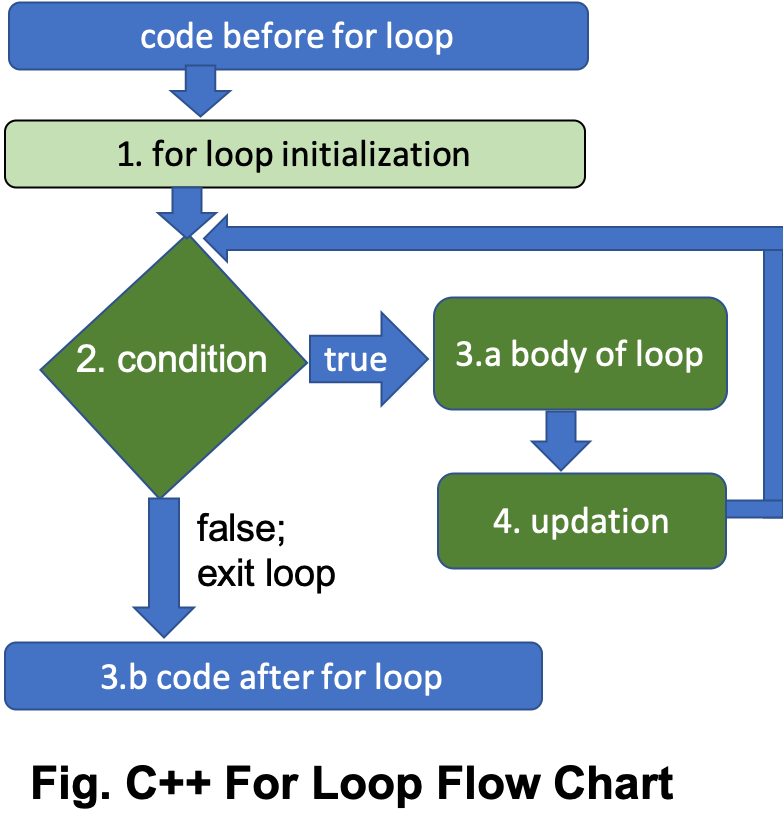
\includegraphics{resources/For-Loop.png}

    \begin{tcolorbox}[breakable, size=fbox, boxrule=1pt, pad at break*=1mm,colback=cellbackground, colframe=cellborder]
\prompt{In}{incolor}{10}{\boxspacing}
\begin{Verbatim}[commandchars=\\\{\}]
\PY{c+c1}{// example 1 \PYZhy{} the hard way of repeating code!}
\PY{c+c1}{// write a program that counts \PYZdq{}Mississippi!\PYZdq{} 10 times}
\PY{c+c1}{// if you didn\PYZsq{}t know loop, one could still do it, rather painfully!}
\PY{c+c1}{// typing one statement at a time for 10 times!}

\PY{c+cp}{\PYZsh{}}\PY{c+cp}{include} \PY{c+cpf}{\PYZlt{}iostream\PYZgt{}}

\PY{k}{using} \PY{k}{namespace} \PY{n+nn}{std}\PY{p}{;}

\PY{n}{cout} \PY{o}{\PYZlt{}}\PY{o}{\PYZlt{}} \PY{l+s}{\PYZdq{}}\PY{l+s}{1. Mississippi!}\PY{l+s+se}{\PYZbs{}n}\PY{l+s}{\PYZdq{}}\PY{p}{;}
\PY{n}{cout} \PY{o}{\PYZlt{}}\PY{o}{\PYZlt{}} \PY{l+s}{\PYZdq{}}\PY{l+s}{2. Mississippi!}\PY{l+s+se}{\PYZbs{}n}\PY{l+s}{\PYZdq{}}\PY{p}{;}
\PY{n}{cout} \PY{o}{\PYZlt{}}\PY{o}{\PYZlt{}} \PY{l+s}{\PYZdq{}}\PY{l+s}{3. Mississippi!}\PY{l+s+se}{\PYZbs{}n}\PY{l+s}{\PYZdq{}}\PY{p}{;}
\PY{n}{cout} \PY{o}{\PYZlt{}}\PY{o}{\PYZlt{}} \PY{l+s}{\PYZdq{}}\PY{l+s}{4. Mississippi!}\PY{l+s+se}{\PYZbs{}n}\PY{l+s}{\PYZdq{}}\PY{p}{;}
\PY{n}{cout} \PY{o}{\PYZlt{}}\PY{o}{\PYZlt{}} \PY{l+s}{\PYZdq{}}\PY{l+s}{5. Mississippi!}\PY{l+s+se}{\PYZbs{}n}\PY{l+s}{\PYZdq{}}\PY{p}{;}
\PY{n}{cout} \PY{o}{\PYZlt{}}\PY{o}{\PYZlt{}} \PY{l+s}{\PYZdq{}}\PY{l+s}{6. Mississippi!}\PY{l+s+se}{\PYZbs{}n}\PY{l+s}{\PYZdq{}}\PY{p}{;}
\PY{n}{cout} \PY{o}{\PYZlt{}}\PY{o}{\PYZlt{}} \PY{l+s}{\PYZdq{}}\PY{l+s}{7. Mississippi!}\PY{l+s+se}{\PYZbs{}n}\PY{l+s}{\PYZdq{}}\PY{p}{;}
\PY{n}{cout} \PY{o}{\PYZlt{}}\PY{o}{\PYZlt{}} \PY{l+s}{\PYZdq{}}\PY{l+s}{8. Mississippi!}\PY{l+s+se}{\PYZbs{}n}\PY{l+s}{\PYZdq{}}\PY{p}{;}
\PY{n}{cout} \PY{o}{\PYZlt{}}\PY{o}{\PYZlt{}} \PY{l+s}{\PYZdq{}}\PY{l+s}{9. Mississippi!}\PY{l+s+se}{\PYZbs{}n}\PY{l+s}{\PYZdq{}}\PY{p}{;}
\PY{n}{cout} \PY{o}{\PYZlt{}}\PY{o}{\PYZlt{}} \PY{l+s}{\PYZdq{}}\PY{l+s}{10. Mississippi!}\PY{l+s+se}{\PYZbs{}n}\PY{l+s}{\PYZdq{}}\PY{p}{;}
\PY{c+c1}{// phew... gets worse, when you need to do it for 100 or 1000 or more times... Yikes!!}
\PY{c+c1}{// you might just quit programming right now!}
\end{Verbatim}
\end{tcolorbox}

    \begin{Verbatim}[commandchars=\\\{\}]
1. Mississippi!
2. Mississippi!
3. Mississippi!
4. Mississippi!
5. Mississippi!
6. Mississippi!
7. Mississippi!
8. Mississippi!
9. Mississippi!
10. Mississippi!
    \end{Verbatim}

            \begin{tcolorbox}[breakable, size=fbox, boxrule=.5pt, pad at break*=1mm, opacityfill=0]
\prompt{Out}{outcolor}{10}{\boxspacing}
\begin{Verbatim}[commandchars=\\\{\}]
@0x10597fed0
\end{Verbatim}
\end{tcolorbox}
        
    \begin{tcolorbox}[breakable, size=fbox, boxrule=1pt, pad at break*=1mm,colback=cellbackground, colframe=cellborder]
\prompt{In}{incolor}{11}{\boxspacing}
\begin{Verbatim}[commandchars=\\\{\}]
\PY{c+c1}{// Let\PYZsq{}s make our life a little easier!}
\PY{c+c1}{// using for loop, let\PYZsq{}s tell the computer to repeatedly print \PYZdq{}Mississippi!\PYZdq{} 10 times }
\PY{c+c1}{// so we don\PYZsq{}t have to type 10 different statements!}
\PY{k}{for}\PY{p}{(}\PY{k+kt}{int} \PY{n}{i}\PY{o}{=}\PY{l+m+mi}{1}\PY{p}{;} \PY{n}{i}\PY{o}{\PYZlt{}}\PY{o}{=}\PY{l+m+mi}{10}\PY{p}{;} \PY{n}{i}\PY{o}{+}\PY{o}{+}\PY{p}{)} \PY{p}{\PYZob{}}
    \PY{c+c1}{// it\PYZsq{}s common practice that i, j, k are used as loop counter variables}
    \PY{c+c1}{// you can use any identifier}
    \PY{n}{cout} \PY{o}{\PYZlt{}}\PY{o}{\PYZlt{}}  \PY{n}{i} \PY{o}{\PYZlt{}}\PY{o}{\PYZlt{}} \PY{l+s}{\PYZdq{}}\PY{l+s}{. Mississippi!}\PY{l+s+se}{\PYZbs{}n}\PY{l+s}{\PYZdq{}}\PY{p}{;}
\PY{p}{\PYZcb{}}
\PY{c+c1}{// how about counting \PYZdq{}Mississippi!\PYZdq{} 100 times or even 1000 and more?}
\end{Verbatim}
\end{tcolorbox}

    \begin{Verbatim}[commandchars=\\\{\}]
1. Mississippi!
2. Mississippi!
3. Mississippi!
4. Mississippi!
5. Mississippi!
6. Mississippi!
7. Mississippi!
8. Mississippi!
9. Mississippi!
10. Mississippi!
    \end{Verbatim}

    \hypertarget{visualize-for-loop-execution-in-pythontutor.com}{%
\subsubsection{\texorpdfstring{visualize for loop execution in
\href{http://pythontutor.com/cpp.html\#code=//\%20for\%20loop\%20visualization\%0A\%23include\%20\%3Ciostream\%3E\%0Ausing\%20namespace\%20std\%3B\%0A\%0Aint\%20main\%28\%29\%20\%7B\%0A\%20\%20cout\%20\%3C\%3C\%20\%22before\%20for\%20loop\%22\%20\%3C\%3C\%20endl\%3B\%0A\%20\%20for\%28int\%20i\%3D1\%3B\%20i\%3C\%3D5\%3B\%20i\%2B\%2B\%29\%0A\%20\%20\%20\%20cout\%20\%3C\%3C\%20i\%20\%3C\%3C\%20\%22.\%20Hello\%20World!\%5Cn\%22\%3B\%0A\%20\%20\%0A\%20\%20cout\%20\%3C\%3C\%20\%22after\%20for\%20loop\%5Cn\%22\%3B\%0A\%20\%20\%0A\%20\%20return\%200\%3B\%0A\%7D\&curInstr=0\&mode=display\&origin=opt-frontend.js\&py=cpp\&rawInputLstJSON=\%5B\%5D}{pythontutor.com}}{visualize for loop execution in pythontutor.com}}\label{visualize-for-loop-execution-in-pythontutor.com}}

\hypertarget{intialization-condition-and-updation-statements-are-optional-and-independent}{%
\subsubsection{intialization, condition and updation statements are
optional and
independent}\label{intialization-condition-and-updation-statements-are-optional-and-independent}}

\begin{itemize}
\tightlist
\item
  the intitialization, condtion and updation expressions in the
  \textbf{for loop} statment are all optional
\item
  these can also have multiple statments separated by comma

  \begin{itemize}
  \tightlist
  \item
    e.g., you can have multiple initialization statements
  \item
    you can have multiple update statements
  \item
    you can have complex logical statement for condition
  \end{itemize}
\end{itemize}

\hypertarget{infinite-loop}{%
\subsubsection{infinite loop}\label{infinite-loop}}

\begin{itemize}
\tightlist
\item
  a common mistake a programmer can make while constructing a loop
\item
  happens when you forget to update the loop counter variable or use
  condition that is always true
\end{itemize}

    \begin{tcolorbox}[breakable, size=fbox, boxrule=1pt, pad at break*=1mm,colback=cellbackground, colframe=cellborder]
\prompt{In}{incolor}{ }{\boxspacing}
\begin{Verbatim}[commandchars=\\\{\}]
\PY{c+c1}{// infinite loop example}
\PY{c+c1}{// if you run this, computer will not stop executing the loop body!}
\PY{c+c1}{// you\PYZsq{}ve to manually interrupt the Kernel in Jupyter notebook}
\PY{c+c1}{// Click Kernel \PYZhy{}\PYZgt{} Inerrrput}
\PY{k}{for}\PY{p}{(} \PY{p}{;} \PY{p}{;} \PY{p}{)} \PY{p}{\PYZob{}} \PY{c+c1}{// infinite loop; no condition that stops the for loop}
    \PY{n}{cout} \PY{o}{\PYZlt{}}\PY{o}{\PYZlt{}} \PY{l+s}{\PYZdq{}}\PY{l+s}{Hello World!}\PY{l+s}{\PYZdq{}} \PY{o}{\PYZlt{}}\PY{o}{\PYZlt{}} \PY{n}{endl}\PY{p}{;}
\PY{p}{\PYZcb{}}
\end{Verbatim}
\end{tcolorbox}

    \begin{tcolorbox}[breakable, size=fbox, boxrule=1pt, pad at break*=1mm,colback=cellbackground, colframe=cellborder]
\prompt{In}{incolor}{1}{\boxspacing}
\begin{Verbatim}[commandchars=\\\{\}]
\PY{c+c1}{// if the kernel restarts; must include all the libraries again}
\PY{c+cp}{\PYZsh{}}\PY{c+cp}{include} \PY{c+cpf}{\PYZlt{}iostream\PYZgt{}}
\PY{k}{using} \PY{k}{namespace} \PY{n+nn}{std}\PY{p}{;}
\end{Verbatim}
\end{tcolorbox}

    \begin{tcolorbox}[breakable, size=fbox, boxrule=1pt, pad at break*=1mm,colback=cellbackground, colframe=cellborder]
\prompt{In}{incolor}{2}{\boxspacing}
\begin{Verbatim}[commandchars=\\\{\}]
\PY{c+c1}{// for loop with multiple statements for initialization; condition and updation}
\PY{k}{for}\PY{p}{(}\PY{k+kt}{int} \PY{n}{i}\PY{o}{=}\PY{l+m+mi}{1}\PY{p}{,} \PY{n}{j}\PY{o}{=}\PY{l+m+mi}{10}\PY{p}{;} \PY{n}{i}\PY{o}{\PYZlt{}}\PY{o}{=}\PY{l+m+mi}{10} \PY{o}{\PYZam{}}\PY{o}{\PYZam{}} \PY{n}{j}\PY{o}{\PYZgt{}}\PY{o}{=}\PY{l+m+mi}{1}\PY{p}{;} \PY{n}{i}\PY{o}{+}\PY{o}{+}\PY{p}{,} \PY{n}{j}\PY{o}{\PYZhy{}}\PY{o}{\PYZhy{}}\PY{p}{)} \PY{p}{\PYZob{}}
    \PY{n}{cout} \PY{o}{\PYZlt{}}\PY{o}{\PYZlt{}} \PY{n}{i} \PY{o}{\PYZlt{}}\PY{o}{\PYZlt{}} \PY{l+s}{\PYZdq{}}\PY{l+s}{ + }\PY{l+s}{\PYZdq{}} \PY{o}{\PYZlt{}}\PY{o}{\PYZlt{}} \PY{n}{j} \PY{o}{\PYZlt{}}\PY{o}{\PYZlt{}} \PY{l+s}{\PYZdq{}}\PY{l+s}{ = }\PY{l+s}{\PYZdq{}} \PY{o}{\PYZlt{}}\PY{o}{\PYZlt{}} \PY{n}{i}\PY{o}{+}\PY{n}{j} \PY{o}{\PYZlt{}}\PY{o}{\PYZlt{}} \PY{n}{endl}\PY{p}{;}
\PY{p}{\PYZcb{}}
\end{Verbatim}
\end{tcolorbox}

    \begin{Verbatim}[commandchars=\\\{\}]
1 + 10 = 11
2 + 9 = 11
3 + 8 = 11
4 + 7 = 11
5 + 6 = 11
6 + 5 = 11
7 + 4 = 11
8 + 3 = 11
9 + 2 = 11
10 + 1 = 11
    \end{Verbatim}

    \hypertarget{break-and-continue}{%
\subsection{\texorpdfstring{\texttt{break} and
\texttt{continue}}{break and continue}}\label{break-and-continue}}

\begin{itemize}
\tightlist
\item
  two commonly used statements inside the loop body
\item
  \texttt{break} statement breaks/exits the loop immidiately when
  executed

  \begin{itemize}
  \tightlist
  \item
    any code after \texttt{break} inside the loop body will be ignored
  \end{itemize}
\item
  \texttt{continue} statement makes next loop or iteration to execute
  immidiately

  \begin{itemize}
  \tightlist
  \item
    any code after \texttt{continue} inside the loop body will be
    skipped
  \end{itemize}
\item
  \texttt{break} and \texttt{continue} are typically used based on some
  condition

  \begin{itemize}
  \tightlist
  \item
    with the reason to exit the loop body or continue with next
    iteration skipping the rest of the loop body
  \end{itemize}
\end{itemize}

    \begin{tcolorbox}[breakable, size=fbox, boxrule=1pt, pad at break*=1mm,colback=cellbackground, colframe=cellborder]
\prompt{In}{incolor}{2}{\boxspacing}
\begin{Verbatim}[commandchars=\\\{\}]
\PY{c+c1}{// example of break and continue}
\PY{c+c1}{// comment and uncomment break and continue to see how each works}
\PY{k}{for}\PY{p}{(}\PY{k+kt}{int} \PY{n}{i}\PY{o}{=}\PY{l+m+mi}{1}\PY{p}{;} \PY{n}{i}\PY{o}{\PYZlt{}}\PY{o}{=}\PY{l+m+mi}{10}\PY{p}{;} \PY{n}{i}\PY{o}{+}\PY{o}{+}\PY{p}{)} \PY{p}{\PYZob{}}
    \PY{n}{cout} \PY{o}{\PYZlt{}}\PY{o}{\PYZlt{}}  \PY{n}{i} \PY{o}{\PYZlt{}}\PY{o}{\PYZlt{}} \PY{l+s}{\PYZdq{}}\PY{l+s}{. Mississippi!}\PY{l+s+se}{\PYZbs{}n}\PY{l+s}{\PYZdq{}}\PY{p}{;}
    \PY{k}{break}\PY{p}{;}
    \PY{n}{cout} \PY{o}{\PYZlt{}}\PY{o}{\PYZlt{}} \PY{n}{i} \PY{o}{\PYZlt{}}\PY{o}{\PYZlt{}} \PY{l+s}{\PYZdq{}}\PY{l+s}{. Hello World!}\PY{l+s+se}{\PYZbs{}n}\PY{l+s}{\PYZdq{}}\PY{p}{;}
    \PY{c+c1}{// continue;}
\PY{p}{\PYZcb{}}
\end{Verbatim}
\end{tcolorbox}

    \begin{Verbatim}[commandchars=\\\{\}]
1. Mississippi!
    \end{Verbatim}

    \begin{tcolorbox}[breakable, size=fbox, boxrule=1pt, pad at break*=1mm,colback=cellbackground, colframe=cellborder]
\prompt{In}{incolor}{3}{\boxspacing}
\begin{Verbatim}[commandchars=\\\{\}]
\PY{c+c1}{// break example}
\PY{n}{cout} \PY{o}{\PYZlt{}}\PY{o}{\PYZlt{}} \PY{l+s}{\PYZdq{}}\PY{l+s}{before loop}\PY{l+s+se}{\PYZbs{}n}\PY{l+s}{\PYZdq{}}\PY{p}{;}
\PY{k}{for}\PY{p}{(}\PY{k+kt}{int} \PY{n}{i}\PY{o}{=}\PY{l+m+mi}{1}\PY{p}{;} \PY{n}{i}\PY{o}{\PYZlt{}}\PY{o}{=}\PY{l+m+mi}{10}\PY{p}{;} \PY{n}{i}\PY{o}{+}\PY{o}{+}\PY{p}{)} \PY{p}{\PYZob{}}
    \PY{k}{if} \PY{p}{(}\PY{n}{i} \PY{o}{=}\PY{o}{=} \PY{l+m+mi}{5}\PY{p}{)}
        \PY{k}{break}\PY{p}{;}
    \PY{n}{cout} \PY{o}{\PYZlt{}}\PY{o}{\PYZlt{}} \PY{n}{i} \PY{o}{\PYZlt{}}\PY{o}{\PYZlt{}} \PY{l+s}{\PYZdq{}}\PY{l+s}{. Hello World!}\PY{l+s}{\PYZdq{}} \PY{o}{\PYZlt{}}\PY{o}{\PYZlt{}} \PY{n}{endl}\PY{p}{;}
\PY{p}{\PYZcb{}}
\PY{n}{cout} \PY{o}{\PYZlt{}}\PY{o}{\PYZlt{}} \PY{l+s}{\PYZdq{}}\PY{l+s}{after loop... all done!}\PY{l+s+se}{\PYZbs{}n}\PY{l+s}{\PYZdq{}}\PY{p}{;}
\end{Verbatim}
\end{tcolorbox}

    \begin{Verbatim}[commandchars=\\\{\}]
before loop
1. Hello World!
2. Hello World!
3. Hello World!
4. Hello World!
after loop{\ldots} all done!
    \end{Verbatim}

    \begin{tcolorbox}[breakable, size=fbox, boxrule=1pt, pad at break*=1mm,colback=cellbackground, colframe=cellborder]
\prompt{In}{incolor}{6}{\boxspacing}
\begin{Verbatim}[commandchars=\\\{\}]
\PY{c+c1}{// continue example}
\PY{c+c1}{// print odd numbers between 1 and 20}
\PY{n}{cout} \PY{o}{\PYZlt{}}\PY{o}{\PYZlt{}} \PY{l+s}{\PYZdq{}}\PY{l+s}{before loop}\PY{l+s+se}{\PYZbs{}n}\PY{l+s}{\PYZdq{}}\PY{p}{;}
\PY{k}{for}\PY{p}{(}\PY{k+kt}{int} \PY{n}{i}\PY{o}{=}\PY{l+m+mi}{1}\PY{p}{;} \PY{n}{i}\PY{o}{\PYZlt{}}\PY{o}{=}\PY{l+m+mi}{20}\PY{p}{;} \PY{n}{i}\PY{o}{+}\PY{o}{+}\PY{p}{)} \PY{p}{\PYZob{}}
    \PY{k}{if} \PY{p}{(}\PY{n}{i}\PY{o}{\PYZpc{}}\PY{l+m+mi}{2} \PY{o}{=}\PY{o}{=} \PY{l+m+mi}{0}\PY{p}{)} \PY{c+c1}{// skip every even i}
        \PY{k}{continue}\PY{p}{;}
    \PY{n}{cout} \PY{o}{\PYZlt{}}\PY{o}{\PYZlt{}} \PY{n}{i} \PY{o}{\PYZlt{}}\PY{o}{\PYZlt{}} \PY{l+s}{\PYZdq{}}\PY{l+s}{ }\PY{l+s}{\PYZdq{}}\PY{p}{;}
\PY{p}{\PYZcb{}}
\PY{n}{cout} \PY{o}{\PYZlt{}}\PY{o}{\PYZlt{}} \PY{l+s}{\PYZdq{}}\PY{l+s+se}{\PYZbs{}n}\PY{l+s}{after loop... all done!}\PY{l+s+se}{\PYZbs{}n}\PY{l+s}{\PYZdq{}}\PY{p}{;}
\end{Verbatim}
\end{tcolorbox}

    \begin{Verbatim}[commandchars=\\\{\}]
before loop
1 3 5 7 9 11 13 15 17 19
after loop{\ldots} all done!
    \end{Verbatim}

    \begin{tcolorbox}[breakable, size=fbox, boxrule=1pt, pad at break*=1mm,colback=cellbackground, colframe=cellborder]
\prompt{In}{incolor}{2}{\boxspacing}
\begin{Verbatim}[commandchars=\\\{\}]
\PY{c+c1}{// breaking infinite loop!}
\PY{k+kt}{int} \PY{n}{i}\PY{o}{=}\PY{l+m+mi}{1}\PY{p}{,} \PY{n}{j}\PY{o}{=}\PY{l+m+mi}{10}\PY{p}{;}
\PY{k}{for}\PY{p}{(} \PY{p}{;} \PY{p}{;} \PY{p}{)} \PY{p}{\PYZob{}} \PY{c+c1}{// you could write int i=1, j=10; as initialization}
    \PY{k}{if} \PY{p}{(}\PY{n}{i}\PY{o}{\PYZlt{}}\PY{o}{=}\PY{l+m+mi}{10} \PY{o}{\PYZam{}}\PY{o}{\PYZam{}} \PY{n}{j}\PY{o}{\PYZgt{}}\PY{o}{=}\PY{l+m+mi}{1}\PY{p}{)}
        \PY{n}{cout} \PY{o}{\PYZlt{}}\PY{o}{\PYZlt{}} \PY{n}{i} \PY{o}{\PYZlt{}}\PY{o}{\PYZlt{}} \PY{l+s}{\PYZdq{}}\PY{l+s}{ + }\PY{l+s}{\PYZdq{}} \PY{o}{\PYZlt{}}\PY{o}{\PYZlt{}} \PY{n}{j} \PY{o}{\PYZlt{}}\PY{o}{\PYZlt{}} \PY{l+s}{\PYZdq{}}\PY{l+s}{ = }\PY{l+s}{\PYZdq{}} \PY{o}{\PYZlt{}}\PY{o}{\PYZlt{}} \PY{n}{i}\PY{o}{+}\PY{n}{j} \PY{o}{\PYZlt{}}\PY{o}{\PYZlt{}} \PY{n}{endl}\PY{p}{;}
    \PY{k}{else}
        \PY{k}{break}\PY{p}{;}
    
    \PY{n}{i}\PY{o}{+}\PY{o}{+}\PY{p}{,} \PY{n}{j}\PY{o}{\PYZhy{}}\PY{o}{\PYZhy{}}\PY{p}{;}
\PY{p}{\PYZcb{}}
\end{Verbatim}
\end{tcolorbox}

    \begin{Verbatim}[commandchars=\\\{\}]
1 + 10 = 11
2 + 9 = 11
3 + 8 = 11
4 + 7 = 11
5 + 6 = 11
6 + 5 = 11
7 + 4 = 11
8 + 3 = 11
9 + 2 = 11
10 + 1 = 11
    \end{Verbatim}

    \begin{tcolorbox}[breakable, size=fbox, boxrule=1pt, pad at break*=1mm,colback=cellbackground, colframe=cellborder]
\prompt{In}{incolor}{5}{\boxspacing}
\begin{Verbatim}[commandchars=\\\{\}]
\PY{c+c1}{// Countdown to Blast\PYZhy{}off using for loop}
\PY{c+cp}{\PYZsh{}}\PY{c+cp}{include} \PY{c+cpf}{\PYZlt{}iostream\PYZgt{}}
\PY{c+cp}{\PYZsh{}}\PY{c+cp}{include} \PY{c+cpf}{\PYZlt{}unistd.h\PYZgt{}}

\PY{k}{using} \PY{k}{namespace} \PY{n+nn}{std}\PY{p}{;}
\end{Verbatim}
\end{tcolorbox}

    \begin{tcolorbox}[breakable, size=fbox, boxrule=1pt, pad at break*=1mm,colback=cellbackground, colframe=cellborder]
\prompt{In}{incolor}{3}{\boxspacing}
\begin{Verbatim}[commandchars=\\\{\}]
\PY{k}{for}\PY{p}{(}\PY{k+kt}{int} \PY{n}{i}\PY{o}{=}\PY{l+m+mi}{10}\PY{p}{;} \PY{n}{i}\PY{o}{\PYZgt{}}\PY{o}{=}\PY{l+m+mi}{0}\PY{p}{;} \PY{n}{i}\PY{o}{\PYZhy{}}\PY{o}{\PYZhy{}}\PY{p}{)} \PY{p}{\PYZob{}}
    \PY{k}{if} \PY{p}{(}\PY{n}{i} \PY{o}{=}\PY{o}{=} \PY{l+m+mi}{0}\PY{p}{)}
        \PY{n}{cout} \PY{o}{\PYZlt{}}\PY{o}{\PYZlt{}} \PY{l+s}{\PYZdq{}}\PY{l+s}{Blast Off!!!}\PY{l+s}{\PYZdq{}} \PY{o}{\PYZlt{}}\PY{o}{\PYZlt{}} \PY{n}{endl}\PY{p}{;}
    \PY{k}{else} \PY{p}{\PYZob{}}
        \PY{n}{cout} \PY{o}{\PYZlt{}}\PY{o}{\PYZlt{}} \PY{n}{i} \PY{o}{\PYZlt{}}\PY{o}{\PYZlt{}} \PY{n}{endl}\PY{p}{;}
        \PY{n}{usleep}\PY{p}{(}\PY{l+m+mi}{1000000}\PY{p}{)}\PY{p}{;} \PY{c+c1}{// sleep for 1e6 microseconds = 1 second }
    \PY{p}{\PYZcb{}}
\PY{p}{\PYZcb{}}
\end{Verbatim}
\end{tcolorbox}

    \begin{Verbatim}[commandchars=\\\{\}]
10
9
8
7
6
5
4
3
2
1
Blast Off!!!
    \end{Verbatim}

    \hypertarget{countdown-demo-program---demosloopscountdowncountdown.cpp}{%
\subsubsection{\texorpdfstring{Countdown demo program -
\url{demos/loops/countdown/countdown.cpp}}{Countdown demo program - demos/loops/countdown/countdown.cpp}}\label{countdown-demo-program---demosloopscountdowncountdown.cpp}}

    \hypertarget{range-based-for-loop}{%
\subsection{Range-based for loop}\label{range-based-for-loop}}

\begin{itemize}
\tightlist
\item
  executes a for loop over a range of values
\item
  typically used with container types such as array, vector, set, etc.

  \begin{itemize}
  \tightlist
  \item
    more readable alternative to the for loop operating over all
    elements in a container
  \end{itemize}
\item
  syntax:
\end{itemize}

\begin{Shaded}
\begin{Highlighting}[]
    \ControlFlowTok{for} \OperatorTok{(}\NormalTok{range\_declaration }\OperatorTok{:}\NormalTok{ range\_expression}\OperatorTok{)} \OperatorTok{\{}
        \CommentTok{// loop body}
    \OperatorTok{\}}
\end{Highlighting}
\end{Shaded}

\begin{itemize}
\tightlist
\item
  \texttt{range\ declaration}:

  \begin{itemize}
  \tightlist
  \item
    declares a range variable, whose type is the type of the element in
    the sequence in range\_expression
  \end{itemize}
\item
  \texttt{range\ expression}:

  \begin{itemize}
  \tightlist
  \item
    represents a suitalbe sequence of elements such as array or
    container with begin and end member functions
  \end{itemize}
\end{itemize}

    \begin{tcolorbox}[breakable, size=fbox, boxrule=1pt, pad at break*=1mm,colback=cellbackground, colframe=cellborder]
\prompt{In}{incolor}{3}{\boxspacing}
\begin{Verbatim}[commandchars=\\\{\}]
\PY{c+c1}{// example of range\PYZhy{}based for loop}
\PY{n}{cout} \PY{o}{\PYZlt{}}\PY{o}{\PYZlt{}} \PY{l+s}{\PYZdq{}}\PY{l+s}{before range\PYZhy{}based loop...}\PY{l+s+se}{\PYZbs{}n}\PY{l+s}{\PYZdq{}}\PY{p}{;}
\PY{k}{for}\PY{p}{(}\PY{k+kt}{int} \PY{n+nl}{num}\PY{p}{:} \PY{p}{\PYZob{}}\PY{l+m+mi}{1}\PY{p}{,} \PY{l+m+mi}{2}\PY{p}{,} \PY{l+m+mi}{4}\PY{p}{,} \PY{l+m+mi}{5}\PY{p}{,} \PY{l+m+mi}{6}\PY{p}{,} \PY{l+m+mi}{8}\PY{p}{,} \PY{l+m+mi}{9}\PY{p}{,} \PY{l+m+mi}{10}\PY{p}{\PYZcb{}}\PY{p}{)} \PY{p}{\PYZob{}}
    \PY{n}{cout} \PY{o}{\PYZlt{}}\PY{o}{\PYZlt{}} \PY{n}{num} \PY{o}{\PYZlt{}}\PY{o}{\PYZlt{}} \PY{l+s}{\PYZdq{}}\PY{l+s}{. Mississippi!}\PY{l+s+se}{\PYZbs{}n}\PY{l+s}{\PYZdq{}}\PY{p}{;}
\PY{p}{\PYZcb{}}
\PY{n}{cout} \PY{o}{\PYZlt{}}\PY{o}{\PYZlt{}} \PY{l+s}{\PYZdq{}}\PY{l+s}{after range\PYZhy{}based loop... all done!}\PY{l+s}{\PYZdq{}}\PY{p}{;}
\end{Verbatim}
\end{tcolorbox}

    \begin{Verbatim}[commandchars=\\\{\}]
before range-based loop{\ldots}
1. Mississippi!
2. Mississippi!
4. Mississippi!
5. Mississippi!
6. Mississippi!
8. Mississippi!
9. Mississippi!
10. Mississippi!
after range-based loop{\ldots} all done!
    \end{Verbatim}

    \begin{tcolorbox}[breakable, size=fbox, boxrule=1pt, pad at break*=1mm,colback=cellbackground, colframe=cellborder]
\prompt{In}{incolor}{7}{\boxspacing}
\begin{Verbatim}[commandchars=\\\{\}]
\PY{c+c1}{// example 2: iterate over each character in string using range\PYZhy{}based loop}
\PY{n}{string} \PY{n}{text} \PY{o}{=} \PY{l+s}{\PYZdq{}}\PY{l+s}{This is a sentence!}\PY{l+s}{\PYZdq{}}\PY{p}{;}
\end{Verbatim}
\end{tcolorbox}

    \begin{tcolorbox}[breakable, size=fbox, boxrule=1pt, pad at break*=1mm,colback=cellbackground, colframe=cellborder]
\prompt{In}{incolor}{11}{\boxspacing}
\begin{Verbatim}[commandchars=\\\{\}]
\PY{c+cp}{\PYZsh{}}\PY{c+cp}{include} \PY{c+cpf}{\PYZlt{}cstring\PYZgt{}}\PY{c+c1}{ // touppper}

\PY{c+c1}{// recall: auto can be used to automatically determine type based on value assigned}
\PY{k}{for}\PY{p}{(}\PY{k}{auto} \PY{n+nl}{ch}\PY{p}{:} \PY{n}{text}\PY{p}{)} \PY{p}{\PYZob{}}
    \PY{n}{cout} \PY{o}{\PYZlt{}}\PY{o}{\PYZlt{}} \PY{n}{ch} \PY{o}{\PYZlt{}}\PY{o}{\PYZlt{}} \PY{l+s}{\PYZdq{}}\PY{l+s}{ \PYZhy{}\PYZgt{} ASCII: }\PY{l+s}{\PYZdq{}} \PY{o}{\PYZlt{}}\PY{o}{\PYZlt{}} \PY{k+kt}{int}\PY{p}{(}\PY{n}{ch}\PY{p}{)} \PY{o}{\PYZlt{}}\PY{o}{\PYZlt{}} \PY{l+s}{\PYZdq{}}\PY{l+s}{ UPPER: }\PY{l+s}{\PYZdq{}} \PY{o}{\PYZlt{}}\PY{o}{\PYZlt{}} \PY{k+kt}{char}\PY{p}{(}\PY{n}{toupper}\PY{p}{(}\PY{n}{ch}\PY{p}{)}\PY{p}{)} \PY{o}{\PYZlt{}}\PY{o}{\PYZlt{}} \PY{n}{endl}\PY{p}{;}
\PY{p}{\PYZcb{}}
\end{Verbatim}
\end{tcolorbox}

    \begin{Verbatim}[commandchars=\\\{\}]
T -> ASCII: 84 UPPER: T
h -> ASCII: 104 UPPER: H
i -> ASCII: 105 UPPER: I
s -> ASCII: 115 UPPER: S
  -> ASCII: 32 UPPER:
i -> ASCII: 105 UPPER: I
s -> ASCII: 115 UPPER: S
  -> ASCII: 32 UPPER:
a -> ASCII: 97 UPPER: A
  -> ASCII: 32 UPPER:
s -> ASCII: 115 UPPER: S
e -> ASCII: 101 UPPER: E
n -> ASCII: 110 UPPER: N
t -> ASCII: 116 UPPER: T
e -> ASCII: 101 UPPER: E
n -> ASCII: 110 UPPER: N
c -> ASCII: 99 UPPER: C
e -> ASCII: 101 UPPER: E
! -> ASCII: 33 UPPER: !
    \end{Verbatim}

    \begin{tcolorbox}[breakable, size=fbox, boxrule=1pt, pad at break*=1mm,colback=cellbackground, colframe=cellborder]
\prompt{In}{incolor}{13}{\boxspacing}
\begin{Verbatim}[commandchars=\\\{\}]
\PY{c+c1}{// convert text into uppercase}
\PY{n}{string} \PY{n}{upper\PYZus{}text} \PY{o}{=} \PY{l+s}{\PYZdq{}}\PY{l+s}{\PYZdq{}}\PY{p}{;} \PY{c+c1}{// variable to collect uppercase characters}
\PY{k}{for}\PY{p}{(}\PY{k}{auto} \PY{n+nl}{ch}\PY{p}{:} \PY{n}{text}\PY{p}{)} \PY{p}{\PYZob{}}
    \PY{n}{upper\PYZus{}text} \PY{o}{+}\PY{o}{=} \PY{k+kt}{char}\PY{p}{(}\PY{n}{toupper}\PY{p}{(}\PY{n}{ch}\PY{p}{)}\PY{p}{)}\PY{p}{;}
\PY{p}{\PYZcb{}}
\PY{n}{cout} \PY{o}{\PYZlt{}}\PY{o}{\PYZlt{}} \PY{n}{text} \PY{o}{\PYZlt{}}\PY{o}{\PYZlt{}} \PY{l+s}{\PYZdq{}}\PY{l+s}{ \PYZhy{}\PYZgt{} }\PY{l+s}{\PYZdq{}} \PY{o}{\PYZlt{}}\PY{o}{\PYZlt{}} \PY{n}{upper\PYZus{}text} \PY{o}{\PYZlt{}}\PY{o}{\PYZlt{}} \PY{n}{endl}\PY{p}{;}
\end{Verbatim}
\end{tcolorbox}

    \begin{Verbatim}[commandchars=\\\{\}]
This is a sentence! -> THIS IS A SENTENCE!
    \end{Verbatim}

    \hypertarget{while-loop}{%
\subsection{while loop}\label{while-loop}}

\begin{itemize}
\tightlist
\item
  \texttt{while} keyword is used to create \texttt{while} statment

  \begin{itemize}
  \tightlist
  \item
    a loop that iterates 0 or more times
  \end{itemize}
\item
  if you're not sure how many times the loop should iterate, you use
  \texttt{while} loop
\item
  while statement can be read as if it were English

  \begin{itemize}
  \tightlist
  \item
    e.g.~while you're not tired, keep running the track
  \item
    as opposed to \texttt{for} loop that says, run the track 10 times
  \end{itemize}
\item
  syntax:
\end{itemize}

\begin{Shaded}
\begin{Highlighting}[]
    \ControlFlowTok{while}\OperatorTok{(}\NormalTok{condition}\OperatorTok{)} \OperatorTok{\{}
        \CommentTok{// body of loop}
    \OperatorTok{\}}
\end{Highlighting}
\end{Shaded}

\begin{itemize}
\tightlist
\item
  execute the body of loop as long as the condition is true
\item
  the following figure depicts while loop execution
\end{itemize}

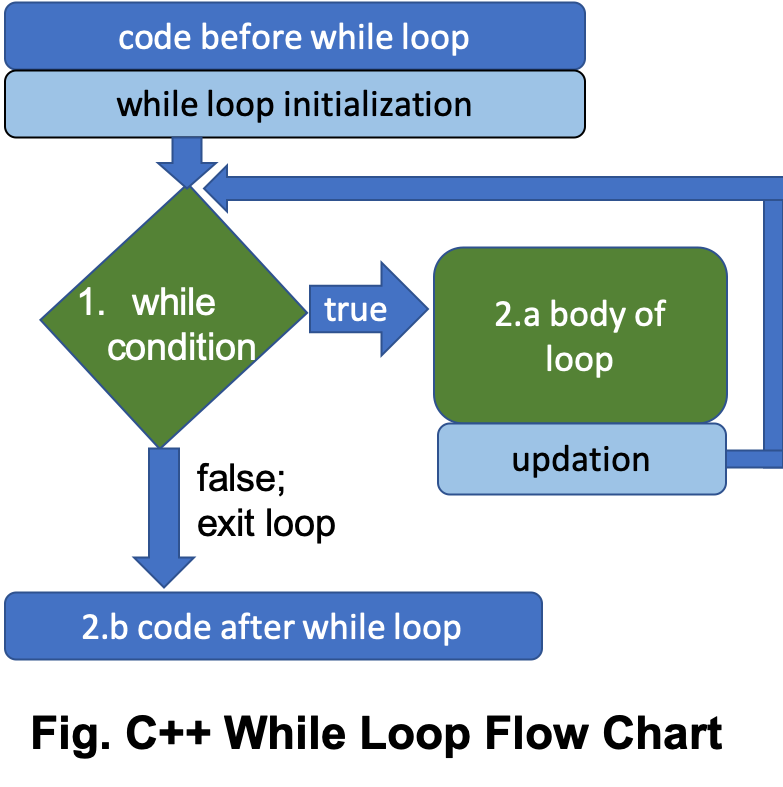
\includegraphics{resources/While-Loop.png}

    \begin{tcolorbox}[breakable, size=fbox, boxrule=1pt, pad at break*=1mm,colback=cellbackground, colframe=cellborder]
\prompt{In}{incolor}{1}{\boxspacing}
\begin{Verbatim}[commandchars=\\\{\}]
\PY{c+c1}{// example 1 \PYZhy{} print a log table from 1 to 10}
\PY{c+cp}{\PYZsh{}}\PY{c+cp}{include} \PY{c+cpf}{\PYZlt{}iostream\PYZgt{}}
\PY{c+cp}{\PYZsh{}}\PY{c+cp}{include} \PY{c+cpf}{\PYZlt{}cmath\PYZgt{}}\PY{c+c1}{ // log, log2, log10}
\PY{c+cp}{\PYZsh{}}\PY{c+cp}{include} \PY{c+cpf}{\PYZlt{}iomanip\PYZgt{}}

\PY{k}{using} \PY{k}{namespace} \PY{n+nn}{std}\PY{p}{;}

\PY{k+kt}{double} \PY{n}{x}\PY{p}{;} \PY{c+c1}{// while loop initialization}
\end{Verbatim}
\end{tcolorbox}

    \begin{tcolorbox}[breakable, size=fbox, boxrule=1pt, pad at break*=1mm,colback=cellbackground, colframe=cellborder]
\prompt{In}{incolor}{2}{\boxspacing}
\begin{Verbatim}[commandchars=\\\{\}]
\PY{n}{cout} \PY{o}{\PYZlt{}}\PY{o}{\PYZlt{}} \PY{l+s}{\PYZdq{}}\PY{l+s}{x}\PY{l+s+se}{\PYZbs{}t}\PY{l+s}{log(x)}\PY{l+s+se}{\PYZbs{}t}\PY{l+s}{log2(x)}\PY{l+s+se}{\PYZbs{}t}\PY{l+s}{log10(x)}\PY{l+s+se}{\PYZbs{}n}\PY{l+s}{\PYZdq{}}\PY{p}{;}
\PY{n}{cout} \PY{o}{\PYZlt{}}\PY{o}{\PYZlt{}} \PY{n}{setw}\PY{p}{(}\PY{l+m+mi}{35}\PY{p}{)} \PY{o}{\PYZlt{}}\PY{o}{\PYZlt{}} \PY{n}{setfill}\PY{p}{(}\PY{l+s+sc}{\PYZsq{}}\PY{l+s+sc}{=}\PY{l+s+sc}{\PYZsq{}}\PY{p}{)} \PY{o}{\PYZlt{}}\PY{o}{\PYZlt{}} \PY{l+s}{\PYZdq{}}\PY{l+s+se}{\PYZbs{}n}\PY{l+s}{\PYZdq{}}\PY{p}{;}
\PY{n}{cout} \PY{o}{\PYZlt{}}\PY{o}{\PYZlt{}} \PY{n}{fixed} \PY{o}{\PYZlt{}}\PY{o}{\PYZlt{}} \PY{n}{setprecision}\PY{p}{(}\PY{l+m+mi}{4}\PY{p}{)}\PY{p}{;}
\PY{n}{x} \PY{o}{=} \PY{l+m+mf}{1.0}\PY{p}{;}
\PY{k}{while}\PY{p}{(}\PY{n}{x} \PY{o}{\PYZlt{}}\PY{o}{=} \PY{l+m+mf}{10.0}\PY{p}{)} \PY{p}{\PYZob{}}
    \PY{c+c1}{// natural log base e, base 2 and base 10}
    \PY{n}{cout} \PY{o}{\PYZlt{}}\PY{o}{\PYZlt{}} \PY{n}{x} \PY{o}{\PYZlt{}}\PY{o}{\PYZlt{}} \PY{l+s+sc}{\PYZsq{}}\PY{l+s+sc}{\PYZbs{}t}\PY{l+s+sc}{\PYZsq{}} \PY{o}{\PYZlt{}}\PY{o}{\PYZlt{}} \PY{n}{log}\PY{p}{(}\PY{n}{x}\PY{p}{)} \PY{o}{\PYZlt{}}\PY{o}{\PYZlt{}} \PY{l+s+sc}{\PYZsq{}}\PY{l+s+sc}{\PYZbs{}t}\PY{l+s+sc}{\PYZsq{}} \PY{o}{\PYZlt{}}\PY{o}{\PYZlt{}} \PY{n}{log2}\PY{p}{(}\PY{n}{x}\PY{p}{)} \PY{o}{\PYZlt{}}\PY{o}{\PYZlt{}} \PY{l+s+sc}{\PYZsq{}}\PY{l+s+sc}{\PYZbs{}t}\PY{l+s+sc}{\PYZsq{}} \PY{o}{\PYZlt{}}\PY{o}{\PYZlt{}} \PY{n}{log10}\PY{p}{(}\PY{n}{x}\PY{p}{)} \PY{o}{\PYZlt{}}\PY{o}{\PYZlt{}} \PY{n}{endl}\PY{p}{;}
    \PY{n}{x} \PY{o}{+}\PY{o}{=} \PY{l+m+mf}{1.0}\PY{p}{;} \PY{c+c1}{// update loop variable}
\PY{p}{\PYZcb{}}
\end{Verbatim}
\end{tcolorbox}

    \begin{Verbatim}[commandchars=\\\{\}]
x       log(x)  log2(x) log10(x)
==================================
1.0000  0.0000  0.0000  0.0000
2.0000  0.6931  1.0000  0.3010
3.0000  1.0986  1.5850  0.4771
4.0000  1.3863  2.0000  0.6021
5.0000  1.6094  2.3219  0.6990
6.0000  1.7918  2.5850  0.7782
7.0000  1.9459  2.8074  0.8451
8.0000  2.0794  3.0000  0.9031
9.0000  2.1972  3.1699  0.9542
10.0000 2.3026  3.3219  1.0000
    \end{Verbatim}

    \begin{tcolorbox}[breakable, size=fbox, boxrule=1pt, pad at break*=1mm,colback=cellbackground, colframe=cellborder]
\prompt{In}{incolor}{2}{\boxspacing}
\begin{Verbatim}[commandchars=\\\{\}]
\PY{c+c1}{// example 2 \PYZhy{} run around the track until you\PYZsq{}re tired}
\PY{k+kt}{int} \PY{n}{lapCount} \PY{o}{=} \PY{l+m+mi}{0}\PY{p}{;}
\PY{n}{string} \PY{n}{tired\PYZus{}response}\PY{p}{;}
\PY{k+kt}{bool} \PY{n}{tired} \PY{o}{=} \PY{n+nb}{false}\PY{p}{;} \PY{c+c1}{// while loop initialization}
\end{Verbatim}
\end{tcolorbox}

    \begin{tcolorbox}[breakable, size=fbox, boxrule=1pt, pad at break*=1mm,colback=cellbackground, colframe=cellborder]
\prompt{In}{incolor}{3}{\boxspacing}
\begin{Verbatim}[commandchars=\\\{\}]
\PY{k}{while}\PY{p}{(}\PY{n}{not} \PY{n}{tired}\PY{p}{)} \PY{p}{\PYZob{}}
    \PY{n}{lapCount} \PY{o}{+}\PY{o}{=} \PY{l+m+mi}{1}\PY{p}{;}
    \PY{n}{cout} \PY{o}{\PYZlt{}}\PY{o}{\PYZlt{}} \PY{l+s}{\PYZdq{}}\PY{l+s}{lap count = }\PY{l+s}{\PYZdq{}} \PY{o}{\PYZlt{}}\PY{o}{\PYZlt{}} \PY{n}{lapCount} \PY{o}{\PYZlt{}}\PY{o}{\PYZlt{}} \PY{n}{endl}\PY{p}{;}
    \PY{n}{cout} \PY{o}{\PYZlt{}}\PY{o}{\PYZlt{}} \PY{l+s}{\PYZdq{}}\PY{l+s}{Are you tired yet? [y|yes] or [n}\PY{l+s+se}{\PYZbs{}n}\PY{l+s}{o]: }\PY{l+s}{\PYZdq{}}\PY{p}{;}
    \PY{n}{cin} \PY{o}{\PYZgt{}}\PY{o}{\PYZgt{}} \PY{n}{tired\PYZus{}response}\PY{p}{;}
    \PY{k}{if} \PY{p}{(}\PY{n}{tired\PYZus{}response} \PY{o}{=}\PY{o}{=} \PY{l+s}{\PYZdq{}}\PY{l+s}{y}\PY{l+s}{\PYZdq{}} \PY{n}{or} \PY{n}{tired\PYZus{}response} \PY{o}{=}\PY{o}{=} \PY{l+s}{\PYZdq{}}\PY{l+s}{yes}\PY{l+s}{\PYZdq{}}\PY{p}{)}
        \PY{n}{tired} \PY{o}{=} \PY{n+nb}{true}\PY{p}{;} \PY{c+c1}{// update loop variable}
\PY{p}{\PYZcb{}}
\end{Verbatim}
\end{tcolorbox}

    \begin{Verbatim}[commandchars=\\\{\}]
lap count = 1
Are you tired yet? [y|yes] or [n
o]: n
lap count = 2
Are you tired yet? [y|yes] or [n
o]: no
lap count = 3
Are you tired yet? [y|yes] or [n
o]: yes
    \end{Verbatim}

    \begin{tcolorbox}[breakable, size=fbox, boxrule=1pt, pad at break*=1mm,colback=cellbackground, colframe=cellborder]
\prompt{In}{incolor}{5}{\boxspacing}
\begin{Verbatim}[commandchars=\\\{\}]
\PY{c+c1}{// using break and continue statements in while loop}
\PY{c+c1}{// NOTE: they don\PYZsq{}t have to be used together!}
\PY{n}{lapCount} \PY{o}{=} \PY{l+m+mi}{0}\PY{p}{;}
\PY{k}{while}\PY{p}{(}\PY{n+nb}{true}\PY{p}{)} \PY{p}{\PYZob{}}
    \PY{n}{lapCount} \PY{o}{+}\PY{o}{=} \PY{l+m+mi}{1}\PY{p}{;}
    \PY{k}{if} \PY{p}{(}\PY{n}{lapCount} \PY{o}{=}\PY{o}{=} \PY{l+m+mi}{2}\PY{p}{)} \PY{k}{continue}\PY{p}{;} \PY{c+c1}{// skip the rest of the code}
    \PY{n}{cout} \PY{o}{\PYZlt{}}\PY{o}{\PYZlt{}} \PY{l+s}{\PYZdq{}}\PY{l+s}{lap count = }\PY{l+s}{\PYZdq{}} \PY{o}{\PYZlt{}}\PY{o}{\PYZlt{}} \PY{n}{lapCount} \PY{o}{\PYZlt{}}\PY{o}{\PYZlt{}} \PY{n}{endl}\PY{p}{;}
    \PY{n}{cout} \PY{o}{\PYZlt{}}\PY{o}{\PYZlt{}} \PY{l+s}{\PYZdq{}}\PY{l+s}{Are you tired yet? [y|yes] or [n}\PY{l+s+se}{\PYZbs{}n}\PY{l+s}{o]: }\PY{l+s}{\PYZdq{}}\PY{p}{;}
    \PY{n}{cin} \PY{o}{\PYZgt{}}\PY{o}{\PYZgt{}} \PY{n}{tired\PYZus{}response}\PY{p}{;}
    \PY{k}{if} \PY{p}{(}\PY{n}{tired\PYZus{}response} \PY{o}{=}\PY{o}{=} \PY{l+s}{\PYZdq{}}\PY{l+s}{y}\PY{l+s}{\PYZdq{}} \PY{n}{or} \PY{n}{tired\PYZus{}response} \PY{o}{=}\PY{o}{=} \PY{l+s}{\PYZdq{}}\PY{l+s}{yes}\PY{l+s}{\PYZdq{}}\PY{p}{)}
        \PY{k}{break}\PY{p}{;}
\PY{p}{\PYZcb{}}
\end{Verbatim}
\end{tcolorbox}

    \begin{Verbatim}[commandchars=\\\{\}]
lap count = 1
Are you tired yet? [y|yes] or [n
o]: n
lap count = 3
Are you tired yet? [y|yes] or [n
o]: no
lap count = 4
Are you tired yet? [y|yes] or [n
o]: yes
    \end{Verbatim}

    \hypertarget{visualize-while-loop-in-pythontutor.com}{%
\subsubsection{\texorpdfstring{visualize while loop in
\href{http://pythontutor.com/cpp.html\#code=//\%20while\%20loop\%20visualization\%0A\%23include\%20\%3Ciostream\%3E\%0Ausing\%20namespace\%20std\%3B\%0A\%0Aint\%20main\%28\%29\%20\%7B\%0A\%20\%20cout\%20\%3C\%3C\%20\%22before\%20while\%20loop\%22\%20\%3C\%3C\%20endl\%3B\%0A\%20\%20int\%20i\%3D\%201\%3B\%0A\%20\%20while\%20\%28i\%20\%3C\%3D\%205\%29\%20\%7B\%0A\%20\%20\%20\%20cout\%20\%3C\%3C\%20i\%20\%3C\%3C\%20\%22.\%20Hello\%20World!\%5Cn\%22\%3B\%0A\%20\%20\%20\%20i\%2B\%2B\%3B\%0A\%20\%20\%7D\%0A\%20\%20\%0A\%20\%20cout\%20\%3C\%3C\%20\%22after\%20while\%20loop\%5Cn\%22\%3B\%0A\%20\%20\%0A\%20\%20return\%200\%3B\%0A\%7D\&curInstr=0\&mode=display\&origin=opt-frontend.js\&py=cpp\&rawInputLstJSON=\%5B\%5D}{pythontutor.com}}{visualize while loop in pythontutor.com}}\label{visualize-while-loop-in-pythontutor.com}}

    \hypertarget{do-while-loop}{%
\subsection{do-while loop}\label{do-while-loop}}

\begin{itemize}
\tightlist
\item
  do while loop is an extension of while loop
\item
  makes a block of code execute 1 or more times
\item
  syntax:
\end{itemize}

\begin{Shaded}
\begin{Highlighting}[]
\ControlFlowTok{do} \OperatorTok{\{}
    \CommentTok{// body of loop}
\OperatorTok{\}} \ControlFlowTok{while} \OperatorTok{(}\NormalTok{condition}\OperatorTok{);}
\end{Highlighting}
\end{Shaded}

\begin{itemize}
\tightlist
\item
  notice the semi-colon after while statement
\item
  interpreting do-while loop

  \begin{enumerate}
  \def\labelenumi{\arabic{enumi}.}
  \tightlist
  \item
    do execute the block of code at least once
  \item
    while the condition is true go to step 1

    \begin{itemize}
    \tightlist
    \item
      exit the loop otherwise
    \end{itemize}
  \end{enumerate}
\item
  the following figure depicts the execution flow of \textbf{do-while
  loop}
\end{itemize}

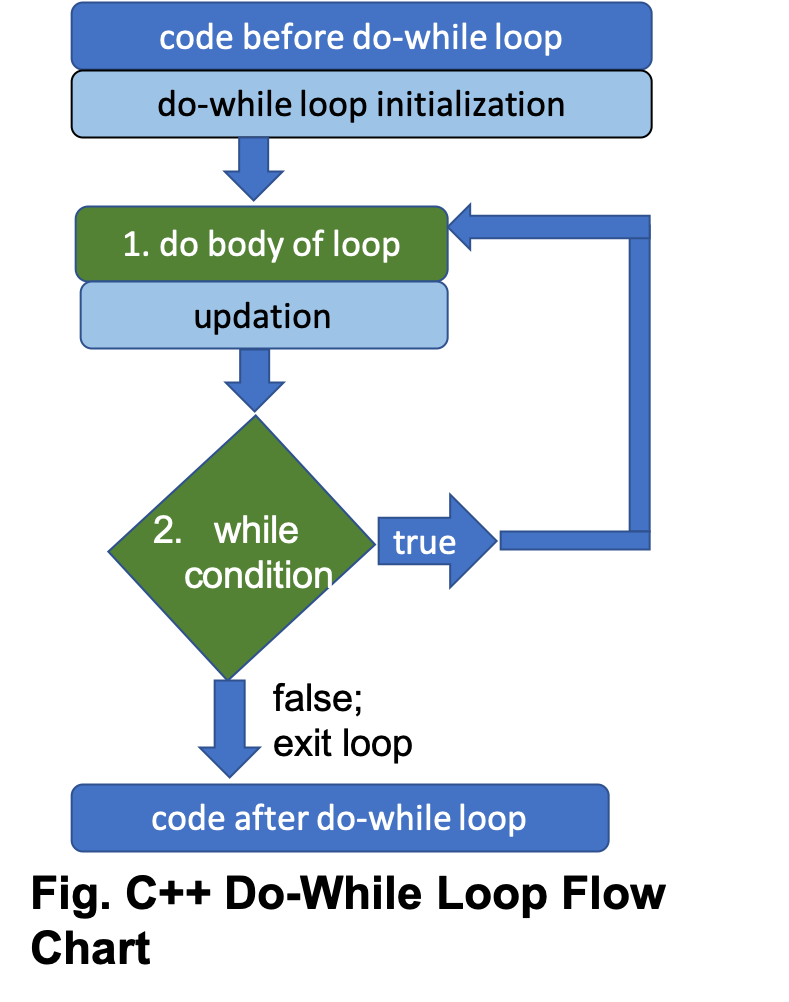
\includegraphics{resources/Do-While-Loop.png}

    \begin{tcolorbox}[breakable, size=fbox, boxrule=1pt, pad at break*=1mm,colback=cellbackground, colframe=cellborder]
\prompt{In}{incolor}{6}{\boxspacing}
\begin{Verbatim}[commandchars=\\\{\}]
\PY{c+c1}{// example 1 \PYZhy{} game play simulation}
\PY{c+c1}{// initialize loop variables}
\PY{k+kt}{int} \PY{n}{counter} \PY{o}{=} \PY{l+m+mi}{0}\PY{p}{;} \PY{c+c1}{// keep track of no. of times game is played}
\PY{n}{string} \PY{n}{play\PYZus{}again}\PY{p}{;} \PY{c+c1}{// player\PYZsq{}s response after each game}
\end{Verbatim}
\end{tcolorbox}

    \begin{tcolorbox}[breakable, size=fbox, boxrule=1pt, pad at break*=1mm,colback=cellbackground, colframe=cellborder]
\prompt{In}{incolor}{7}{\boxspacing}
\begin{Verbatim}[commandchars=\\\{\}]
\PY{c+c1}{// play game at least once}
\PY{k}{do} \PY{p}{\PYZob{}}
    \PY{c+c1}{// call game() function or implement game here...}
    \PY{n}{counter}\PY{o}{+}\PY{o}{+}\PY{p}{;}
    \PY{n}{cout} \PY{o}{\PYZlt{}}\PY{o}{\PYZlt{}} \PY{l+s}{\PYZdq{}}\PY{l+s}{played }\PY{l+s}{\PYZdq{}} \PY{o}{\PYZlt{}}\PY{o}{\PYZlt{}} \PY{n}{counter} \PY{o}{\PYZlt{}}\PY{o}{\PYZlt{}} \PY{l+s}{\PYZdq{}}\PY{l+s}{ times.}\PY{l+s+se}{\PYZbs{}n}\PY{l+s}{\PYZdq{}}\PY{p}{;}
    \PY{n}{cout} \PY{o}{\PYZlt{}}\PY{o}{\PYZlt{}} \PY{l+s}{\PYZdq{}}\PY{l+s}{want to play again? [y|n]: }\PY{l+s}{\PYZdq{}}\PY{p}{;}
    \PY{n}{cin} \PY{o}{\PYZgt{}}\PY{o}{\PYZgt{}} \PY{n}{play\PYZus{}again}\PY{p}{;}
    \PY{k}{if} \PY{p}{(}\PY{n}{play\PYZus{}again} \PY{o}{!}\PY{o}{=} \PY{l+s}{\PYZdq{}}\PY{l+s}{y}\PY{l+s}{\PYZdq{}}\PY{p}{)} \PY{k}{break}\PY{p}{;}
    \PY{k}{else} \PY{k}{continue}\PY{p}{;} \PY{c+c1}{// not necessary!}
\PY{p}{\PYZcb{}} \PY{k}{while} \PY{p}{(}\PY{n+nb}{true}\PY{p}{)}\PY{p}{;}
\end{Verbatim}
\end{tcolorbox}

    \begin{Verbatim}[commandchars=\\\{\}]
played 1 times.
want to play again? [y|n]: y
played 2 times.
want to play again? [y|n]: y
played 3 times.
want to play again? [y|n]: n
    \end{Verbatim}

    \begin{tcolorbox}[breakable, size=fbox, boxrule=1pt, pad at break*=1mm,colback=cellbackground, colframe=cellborder]
\prompt{In}{incolor}{1}{\boxspacing}
\begin{Verbatim}[commandchars=\\\{\}]
\PY{c+c1}{// example 2 \PYZhy{} input validation}
\PY{k+kt}{int} \PY{n}{input}\PY{p}{;} \PY{c+c1}{// variable to store user input}
\end{Verbatim}
\end{tcolorbox}

    \begin{tcolorbox}[breakable, size=fbox, boxrule=1pt, pad at break*=1mm,colback=cellbackground, colframe=cellborder]
\prompt{In}{incolor}{6}{\boxspacing}
\begin{Verbatim}[commandchars=\\\{\}]
\PY{k}{do} \PY{p}{\PYZob{}}
    \PY{n}{cout} \PY{o}{\PYZlt{}}\PY{o}{\PYZlt{}} \PY{l+s}{\PYZdq{}}\PY{l+s}{Enter a whole number between 1 and 20: }\PY{l+s}{\PYZdq{}}\PY{p}{;}
    \PY{n}{cin} \PY{o}{\PYZgt{}}\PY{o}{\PYZgt{}} \PY{n}{input}\PY{p}{;}
    \PY{k}{if} \PY{p}{(}\PY{n}{cin}\PY{p}{.}\PY{n}{fail}\PY{p}{(}\PY{p}{)}\PY{p}{)} \PY{p}{\PYZob{}} \PY{c+c1}{// somehow cin failed; wrong type is entered}
        \PY{n}{cin}\PY{p}{.}\PY{n}{clear}\PY{p}{(}\PY{p}{)}\PY{p}{;} \PY{c+c1}{// clear the error flag}
        \PY{n}{cin}\PY{p}{.}\PY{n}{ignore}\PY{p}{(}\PY{n}{INT\PYZus{}MAX}\PY{p}{,} \PY{l+s+sc}{\PYZsq{}}\PY{l+s+sc}{\PYZbs{}n}\PY{l+s+sc}{\PYZsq{}}\PY{p}{)}\PY{p}{;} \PY{c+c1}{// extract and discard upto INT\PYZus{}MAX characters or upto \PYZsq{}\PYZbs{}n\PYZsq{} in std input stream}
        \PY{n}{cout} \PY{o}{\PYZlt{}}\PY{o}{\PYZlt{}} \PY{l+s}{\PYZdq{}}\PY{l+s}{Invalid input. Try again!}\PY{l+s+se}{\PYZbs{}n}\PY{l+s}{\PYZdq{}}\PY{p}{;}
        \PY{k}{continue}\PY{p}{;}
    \PY{p}{\PYZcb{}}
    \PY{k}{else} \PY{k}{if} \PY{p}{(}\PY{n}{input} \PY{o}{\PYZlt{}} \PY{l+m+mi}{1} \PY{o}{|}\PY{o}{|} \PY{n}{input} \PY{o}{\PYZgt{}} \PY{l+m+mi}{20}\PY{p}{)} \PY{p}{\PYZob{}}
        \PY{n}{cout} \PY{o}{\PYZlt{}}\PY{o}{\PYZlt{}} \PY{l+s}{\PYZdq{}}\PY{l+s}{input must be a whole number between 1 and 20}\PY{l+s+se}{\PYZbs{}n}\PY{l+s}{\PYZdq{}}\PY{p}{;}
    \PY{p}{\PYZcb{}}
    \PY{k}{else} \PY{k}{break}\PY{p}{;}
\PY{p}{\PYZcb{}} \PY{k}{while} \PY{p}{(}\PY{n+nb}{true}\PY{p}{)}\PY{p}{;}
\end{Verbatim}
\end{tcolorbox}

    \begin{Verbatim}[commandchars=\\\{\}]
Enter a whole number between 1 and 20: -1
input must be a whole number between 1 and 20
Enter a whole number between 1 and 20: 21
input must be a whole number between 1 and 20
Enter a whole number between 1 and 20: asdf
Invalid input. Try again!
Enter a whole number between 1 and 20: sdfaf12
Invalid input. Try again!
Enter a whole number between 1 and 20: 15
    \end{Verbatim}

    \begin{tcolorbox}[breakable, size=fbox, boxrule=1pt, pad at break*=1mm,colback=cellbackground, colframe=cellborder]
\prompt{In}{incolor}{7}{\boxspacing}
\begin{Verbatim}[commandchars=\\\{\}]
\PY{n}{cout} \PY{o}{\PYZlt{}}\PY{o}{\PYZlt{}} \PY{l+s}{\PYZdq{}}\PY{l+s}{Great! You entered: }\PY{l+s}{\PYZdq{}} \PY{o}{\PYZlt{}}\PY{o}{\PYZlt{}} \PY{n}{input} \PY{o}{\PYZlt{}}\PY{o}{\PYZlt{}} \PY{n}{endl}\PY{p}{;}
\end{Verbatim}
\end{tcolorbox}

    \begin{Verbatim}[commandchars=\\\{\}]
Great! You entered: 15
    \end{Verbatim}

    \hypertarget{see-example-2-input-validation-as-a-function-here-demosloopsinput_validateinput_validation.cpp}{%
\subsubsection{\texorpdfstring{see example 2 input validation as a
function here
\url{demos/loops/input_validate/input_validation.cpp}}{see example 2 input validation as a function here demos/loops/input\_validate/input\_validation.cpp}}\label{see-example-2-input-validation-as-a-function-here-demosloopsinput_validateinput_validation.cpp}}

\hypertarget{loops-and-functions}{%
\subsection{Loops and functions}\label{loops-and-functions}}

\begin{itemize}
\tightlist
\item
  all the loop statements can be used inside a function
\item
  in fact, any fundamental concepts (io, math, operations, conditionals,
  loops, etc.) can be used inside loop and function
\item
  functions can be called inside loop body
\end{itemize}

    \hypertarget{write-a-function-that-prints-a-multiplication-table-from-1-to-10-as-shown-below}{%
\subsubsection{write a function that prints a multiplication table from
1 to 10 as shown
below}\label{write-a-function-that-prints-a-multiplication-table-from-1-to-10-as-shown-below}}

\begin{itemize}
\tightlist
\item
  use composition and incremental development
\end{itemize}

\begin{verbatim}
    1    2    3    4    5    6    7    8    9   10
    2    4    6    8   10   12   14   16   18   20
    3    6    9   12   15   18   21   24   27   30
    4    8   12   16   20   24   28   32   36   40
    5   10   15   20   25   30   35   40   45   50
    6   12   18   24   30   36   42   48   54   60
    7   14   21   28   35   42   49   56   63   70
    8   16   24   32   40   48   56   64   72   80
    9   18   27   36   45   54   63   72   81   90
   10   20   30   40   50   60   70   80   90  100
\end{verbatim}

    \begin{tcolorbox}[breakable, size=fbox, boxrule=1pt, pad at break*=1mm,colback=cellbackground, colframe=cellborder]
\prompt{In}{incolor}{3}{\boxspacing}
\begin{Verbatim}[commandchars=\\\{\}]
\PY{c+cp}{\PYZsh{}}\PY{c+cp}{include} \PY{c+cpf}{\PYZlt{}iostream\PYZgt{}}
\PY{c+cp}{\PYZsh{}}\PY{c+cp}{include} \PY{c+cpf}{\PYZlt{}iomanip\PYZgt{}}

\PY{k}{using} \PY{k}{namespace} \PY{n+nn}{std}\PY{p}{;}
\end{Verbatim}
\end{tcolorbox}

    \begin{tcolorbox}[breakable, size=fbox, boxrule=1pt, pad at break*=1mm,colback=cellbackground, colframe=cellborder]
\prompt{In}{incolor}{1}{\boxspacing}
\begin{Verbatim}[commandchars=\\\{\}]
\PY{c+c1}{// function that multiplies two numbers}
\PY{k+kt}{int} \PY{n+nf}{multiply}\PY{p}{(}\PY{k+kt}{int} \PY{n}{n1}\PY{p}{,} \PY{k+kt}{int} \PY{n}{n2}\PY{p}{)} \PY{p}{\PYZob{}}
    \PY{k}{return} \PY{n}{n1}\PY{o}{*}\PY{n}{n2}\PY{p}{;}
\PY{p}{\PYZcb{}}
\end{Verbatim}
\end{tcolorbox}

    \begin{tcolorbox}[breakable, size=fbox, boxrule=1pt, pad at break*=1mm,colback=cellbackground, colframe=cellborder]
\prompt{In}{incolor}{4}{\boxspacing}
\begin{Verbatim}[commandchars=\\\{\}]
\PY{c+c1}{// function prints multiples of N from 1 to 10}
\PY{k+kt}{void} \PY{n+nf}{print\PYZus{}multiples}\PY{p}{(}\PY{k+kt}{int} \PY{n}{N}\PY{p}{)} \PY{p}{\PYZob{}}
    \PY{k}{for}\PY{p}{(}\PY{k+kt}{int} \PY{n}{i}\PY{o}{=}\PY{l+m+mi}{1}\PY{p}{;} \PY{n}{i}\PY{o}{\PYZlt{}}\PY{o}{=}\PY{l+m+mi}{10}\PY{p}{;} \PY{n}{i}\PY{o}{+}\PY{o}{+}\PY{p}{)}
        \PY{n}{cout} \PY{o}{\PYZlt{}}\PY{o}{\PYZlt{}} \PY{n}{setw}\PY{p}{(}\PY{l+m+mi}{5}\PY{p}{)} \PY{o}{\PYZlt{}}\PY{o}{\PYZlt{}} \PY{n}{multiply}\PY{p}{(}\PY{n}{N}\PY{p}{,} \PY{n}{i}\PY{p}{)}\PY{p}{;}
    \PY{n}{cout} \PY{o}{\PYZlt{}}\PY{o}{\PYZlt{}} \PY{n}{endl}\PY{p}{;}
\PY{p}{\PYZcb{}}
\end{Verbatim}
\end{tcolorbox}

    \begin{tcolorbox}[breakable, size=fbox, boxrule=1pt, pad at break*=1mm,colback=cellbackground, colframe=cellborder]
\prompt{In}{incolor}{5}{\boxspacing}
\begin{Verbatim}[commandchars=\\\{\}]
\PY{n}{print\PYZus{}multiples}\PY{p}{(}\PY{l+m+mi}{1}\PY{p}{)}\PY{p}{;}
\end{Verbatim}
\end{tcolorbox}

    \begin{Verbatim}[commandchars=\\\{\}]
    1    2    3    4    5    6    7    8    9   10
    \end{Verbatim}

    \begin{tcolorbox}[breakable, size=fbox, boxrule=1pt, pad at break*=1mm,colback=cellbackground, colframe=cellborder]
\prompt{In}{incolor}{6}{\boxspacing}
\begin{Verbatim}[commandchars=\\\{\}]
\PY{n}{print\PYZus{}multiples}\PY{p}{(}\PY{l+m+mi}{2}\PY{p}{)}\PY{p}{;}
\end{Verbatim}
\end{tcolorbox}

    \begin{Verbatim}[commandchars=\\\{\}]
    2    4    6    8   10   12   14   16   18   20
    \end{Verbatim}

    \begin{tcolorbox}[breakable, size=fbox, boxrule=1pt, pad at break*=1mm,colback=cellbackground, colframe=cellborder]
\prompt{In}{incolor}{7}{\boxspacing}
\begin{Verbatim}[commandchars=\\\{\}]
\PY{c+c1}{// now print\PYZus{}mutiples need to be called 10 times}
\PY{c+c1}{// print\PYZus{}multiples function is used as an inner loop}
\PY{k+kt}{void} \PY{n+nf}{printMultipleTable}\PY{p}{(}\PY{p}{)} \PY{p}{\PYZob{}}
    \PY{k}{for}\PY{p}{(}\PY{k+kt}{int} \PY{n}{i}\PY{o}{=}\PY{l+m+mi}{1}\PY{p}{;} \PY{n}{i}\PY{o}{\PYZlt{}}\PY{o}{=}\PY{l+m+mi}{10}\PY{p}{;} \PY{n}{i}\PY{o}{+}\PY{o}{+}\PY{p}{)}
        \PY{n}{print\PYZus{}multiples}\PY{p}{(}\PY{n}{i}\PY{p}{)}\PY{p}{;}
\PY{p}{\PYZcb{}}
\end{Verbatim}
\end{tcolorbox}

    \begin{tcolorbox}[breakable, size=fbox, boxrule=1pt, pad at break*=1mm,colback=cellbackground, colframe=cellborder]
\prompt{In}{incolor}{8}{\boxspacing}
\begin{Verbatim}[commandchars=\\\{\}]
\PY{n}{printMultipleTable}\PY{p}{(}\PY{p}{)}\PY{p}{;}
\end{Verbatim}
\end{tcolorbox}

    \begin{Verbatim}[commandchars=\\\{\}]
    1    2    3    4    5    6    7    8    9   10
    2    4    6    8   10   12   14   16   18   20
    3    6    9   12   15   18   21   24   27   30
    4    8   12   16   20   24   28   32   36   40
    5   10   15   20   25   30   35   40   45   50
    6   12   18   24   30   36   42   48   54   60
    7   14   21   28   35   42   49   56   63   70
    8   16   24   32   40   48   56   64   72   80
    9   18   27   36   45   54   63   72   81   90
   10   20   30   40   50   60   70   80   90  100
    \end{Verbatim}

    \hypertarget{nested-loops}{%
\subsection{Nested loops}\label{nested-loops}}

\begin{itemize}
\tightlist
\item
  a loop can be nested inside another
\item
  outer loop repeats everything inside inner loop
\item
  a lot of advanced algorithms and problems require many nested double
  and even tripple loops
\end{itemize}

    \begin{tcolorbox}[breakable, size=fbox, boxrule=1pt, pad at break*=1mm,colback=cellbackground, colframe=cellborder]
\prompt{In}{incolor}{9}{\boxspacing}
\begin{Verbatim}[commandchars=\\\{\}]
\PY{c+c1}{// function prints multiplication table using nested loop}
\PY{c+c1}{// print\PYZus{}multiples function is replaced with its actual code}
\PY{k+kt}{void} \PY{n+nf}{multiplicationTable}\PY{p}{(}\PY{p}{)} \PY{p}{\PYZob{}}
    \PY{k}{for}\PY{p}{(}\PY{k+kt}{int} \PY{n}{i}\PY{o}{=}\PY{l+m+mi}{1}\PY{p}{;} \PY{n}{i}\PY{o}{\PYZlt{}}\PY{o}{=}\PY{l+m+mi}{10}\PY{p}{;} \PY{n}{i}\PY{o}{+}\PY{o}{+}\PY{p}{)} \PY{p}{\PYZob{}} \PY{c+c1}{// for each i... (row)}
        \PY{k}{for}\PY{p}{(}\PY{k+kt}{int} \PY{n}{j}\PY{o}{=}\PY{l+m+mi}{1}\PY{p}{;} \PY{n}{j}\PY{o}{\PYZlt{}}\PY{o}{=}\PY{l+m+mi}{10}\PY{p}{;} \PY{n}{j}\PY{o}{+}\PY{o}{+}\PY{p}{)} \PY{c+c1}{// for each column}
            \PY{n}{cout} \PY{o}{\PYZlt{}}\PY{o}{\PYZlt{}} \PY{n}{setw}\PY{p}{(}\PY{l+m+mi}{5}\PY{p}{)} \PY{o}{\PYZlt{}}\PY{o}{\PYZlt{}} \PY{n}{multiply}\PY{p}{(}\PY{n}{i}\PY{p}{,} \PY{n}{j}\PY{p}{)}\PY{p}{;}
        \PY{n}{cout} \PY{o}{\PYZlt{}}\PY{o}{\PYZlt{}} \PY{n}{endl}\PY{p}{;}
    \PY{p}{\PYZcb{}}
\PY{p}{\PYZcb{}}
\end{Verbatim}
\end{tcolorbox}

    \begin{tcolorbox}[breakable, size=fbox, boxrule=1pt, pad at break*=1mm,colback=cellbackground, colframe=cellborder]
\prompt{In}{incolor}{10}{\boxspacing}
\begin{Verbatim}[commandchars=\\\{\}]
\PY{n}{multiplicationTable}\PY{p}{(}\PY{p}{)}\PY{p}{;}
\end{Verbatim}
\end{tcolorbox}

    \begin{Verbatim}[commandchars=\\\{\}]
    1    2    3    4    5    6    7    8    9   10
    2    4    6    8   10   12   14   16   18   20
    3    6    9   12   15   18   21   24   27   30
    4    8   12   16   20   24   28   32   36   40
    5   10   15   20   25   30   35   40   45   50
    6   12   18   24   30   36   42   48   54   60
    7   14   21   28   35   42   49   56   63   70
    8   16   24   32   40   48   56   64   72   80
    9   18   27   36   45   54   63   72   81   90
   10   20   30   40   50   60   70   80   90  100
    \end{Verbatim}

    \hypertarget{define-a-function-that-prints-a-right-traingle-shape-with-some-symbol-such-as-of-given-height-n}{%
\subsubsection{Define a function that prints a right-traingle shape with
some symbol such as * of given height
N}\label{define-a-function-that-prints-a-right-traingle-shape-with-some-symbol-such-as-of-given-height-n}}

\begin{itemize}
\tightlist
\item
  e.g.~the following is a right triangle of height 5 printed with
  \texttt{*}
\end{itemize}

\begin{verbatim}
    * 
    * * 
    * * * 
    * * * * 
    * * * * * 
\end{verbatim}

    \begin{tcolorbox}[breakable, size=fbox, boxrule=1pt, pad at break*=1mm,colback=cellbackground, colframe=cellborder]
\prompt{In}{incolor}{15}{\boxspacing}
\begin{Verbatim}[commandchars=\\\{\}]
\PY{c+c1}{// solution}
\PY{k+kt}{void} \PY{n+nf}{printTriangle}\PY{p}{(}\PY{k+kt}{char} \PY{n}{ch}\PY{p}{,} \PY{k+kt}{int} \PY{n}{height}\PY{p}{)} \PY{p}{\PYZob{}}
    \PY{k}{for}\PY{p}{(}\PY{k+kt}{int} \PY{n}{i}\PY{o}{=}\PY{l+m+mi}{1}\PY{p}{;} \PY{n}{i}\PY{o}{\PYZlt{}}\PY{o}{=}\PY{n}{height}\PY{p}{;} \PY{n}{i}\PY{o}{+}\PY{o}{+}\PY{p}{)} \PY{p}{\PYZob{}} \PY{c+c1}{// could you start i from 0?}
        \PY{k}{for}\PY{p}{(}\PY{k+kt}{int} \PY{n}{j}\PY{o}{=}\PY{l+m+mi}{1}\PY{p}{;} \PY{n}{j}\PY{o}{\PYZlt{}}\PY{o}{=}\PY{n}{i}\PY{p}{;} \PY{n}{j}\PY{o}{+}\PY{o}{+}\PY{p}{)}
            \PY{n}{cout} \PY{o}{\PYZlt{}}\PY{o}{\PYZlt{}} \PY{n}{ch} \PY{o}{\PYZlt{}}\PY{o}{\PYZlt{}} \PY{l+s}{\PYZdq{}}\PY{l+s}{ }\PY{l+s}{\PYZdq{}}\PY{p}{;}
        \PY{n}{cout} \PY{o}{\PYZlt{}}\PY{o}{\PYZlt{}} \PY{n}{endl}\PY{p}{;}
    \PY{p}{\PYZcb{}}
\PY{p}{\PYZcb{}}
\end{Verbatim}
\end{tcolorbox}

    \begin{tcolorbox}[breakable, size=fbox, boxrule=1pt, pad at break*=1mm,colback=cellbackground, colframe=cellborder]
\prompt{In}{incolor}{16}{\boxspacing}
\begin{Verbatim}[commandchars=\\\{\}]
\PY{c+c1}{// call the function to manually test it}
\PY{n}{printTriangle}\PY{p}{(}\PY{l+s+sc}{\PYZsq{}}\PY{l+s+sc}{*}\PY{l+s+sc}{\PYZsq{}}\PY{p}{,} \PY{l+m+mi}{5}\PY{p}{)}\PY{p}{;}
\end{Verbatim}
\end{tcolorbox}

    \begin{Verbatim}[commandchars=\\\{\}]
*
* *
* * *
* * * *
* * * * *
    \end{Verbatim}

    \hypertarget{rectanlge---demo-program}{%
\subsubsection{Rectanlge - demo
program}\label{rectanlge---demo-program}}

\begin{itemize}
\tightlist
\item
  Write a complete C++ that computes area and perimeter of a rectangle
  given length and width
\item
  write at least 3 test cases for each function
\item
  program must calculate area and perimeter of as many rentangles as the
  user wants
\item
  see sample solution here: \url{demos/loops/rectangle/}
\end{itemize}

    \hypertarget{labs}{%
\subsection{Labs}\label{labs}}

\begin{enumerate}
\def\labelenumi{\arabic{enumi}.}
\tightlist
\item
  The following lab demonstrates the use of loop structures in C++ by
  drawing various geometric shapes with ASCII characters.

  \begin{itemize}
  \tightlist
  \item
    Use the code stub in \texttt{loops.cpp} file in
    \href{./labs/loops/}{labs/loops} as a hint to complete the program
  \item
    Use Makefile to compile and build the program
  \item
    Fix all the FIXMEs and write FIXED next to each fixme once fixed
  \end{itemize}
\end{enumerate}

    \hypertarget{exercises}{%
\subsection{Exercises}\label{exercises}}

\begin{enumerate}
\def\labelenumi{\arabic{enumi}.}
\item
  Write a function that prints multiplication table from 1 to some value
  N.

  \begin{itemize}
  \tightlist
  \item
    program only prints the lower half of the table ignoring all the
    redundant upper half values
  \end{itemize}
\item
  Write a C++ program including algorithm steps that calculates area and
  circumference of a circle.

  \begin{itemize}
  \tightlist
  \item
    must write functions to compute area and perimeter and automatically
    test each function with atleast 3 test cases
  \item
    \textbf{program finds area and perimeter of as many circle as the
    user wishes}
  \end{itemize}
\item
  Write a C++ program including algorithm steps that calculates Body
  Mass Index (BMI) of a person.

  \begin{itemize}
  \tightlist
  \item
    must use as many functions as possible
  \item
    write at least 3 test cases for each function
  \item
    more info on BMI -
    https://www.nhlbi.nih.gov/health/educational/lose\_wt/BMI/bmicalc.htm
  \item
    formula found
    \href{https://www.cdc.gov/healthyweight/assessing/bmi/childrens_bmi/childrens_bmi_formula.html\#:~:text=The\%20formula\%20for\%20BMI\%20is,to\%20convert\%20this\%20to\%20meters.\&text=When\%20using\%20English\%20measurements\%2C\%20pounds\%20should\%20be\%20divided\%20by\%20inches\%20squared}{here}
  \item
    \textbf{program must calculate BMI of as many patients as user
    wants}
  \item
    a sample solution is provided at
    \url{exercises/loops/BMI/BMI_v4.cpp}
  \end{itemize}
\item
  Write a C++ program including algorithm steps that computes area and
  perimeter of a triangle given three sides.

  \begin{itemize}
  \tightlist
  \item
    must write and use separate functions to calculate area and
    perimeter
  \item
    write at least 3 test cases for each function
  \item
    \textbf{program computes area and perimeter of as many triangles as
    user wishes}
  \item
    Hint: use Heron's formula to find area with three sides
  \end{itemize}
\item
  Write a C++ program that converts hours into seconds.

  \begin{itemize}
  \tightlist
  \item
    must write and use function(s) to computer answer(s)
  \item
    must write at least 3 test cases for each function
  \item
    e.g.~given 2 hours, program should print 7200 as answer
  \item
    \textbf{program continues to run converting as many hours into
    seconds as the user wishes without restaring it}
  \end{itemize}
\item
  Write a C++ program that converts seconds into hours, minutes and
  seconds.

  \begin{itemize}
  \tightlist
  \item
    must define and use function(s)
  \item
    write at least 3 test cases for each function
  \item
    sample input: 3600 sample output: 1 hour, 0 minute and 0 second
  \item
    sample input: 3661 sample output: 1 hour, 1 minute and 1 second
  \item
    Hint: use series of division and module operations \textbf{program
    will continue to run converting multiple inputs}
  \end{itemize}
\item
  Write a C++ program that counts a number of even digits in a given
  integer.

  \begin{itemize}
  \tightlist
  \item
    must write function and write atleast 3 test cases
  \item
    \textbf{program must continue to run as many times as the user
    wishes}
  \end{itemize}
\item
  Write a C++ program that converts decimal number into binary. See
  Chapter 2 and 3 for the algorithm and partial solution.

  \begin{itemize}
  \tightlist
  \item
    \textbf{program will continue to run converting as many decmial
    number as the user wishes}
  \end{itemize}
\item
  Write a C++ program that converts binary number into decimal. See
  Chapter 2 and 3 for the algorithm.
\item
  Write a C++ program that determines if the given integer is prime.
\item
  Write a C++ program that does countdown for rocket launch. Must use
  for loop.

  \begin{itemize}
  \tightlist
  \item
    prints count down from 10 to 1 and finally prints ``Blast Off!''
  \end{itemize}
\item
  Write a C++ program that does countdown for rocket launch. Must use
  while loop.

  \begin{itemize}
  \tightlist
  \item
    prints count down from 10 to 1 and finally prints ``Blast Off!''
  \end{itemize}
\item
  Write a program that prints a right-traingle shape with some symbol
  such as * and given height N

  \begin{itemize}
  \tightlist
  \item
    e.g.~the following is a righ-right triangle of height 5 printed with
    *
  \end{itemize}
\end{enumerate}

\begin{verbatim}
* * * * *
* * * *
* * * 
* *  
* 
\end{verbatim}

\begin{enumerate}
\def\labelenumi{\arabic{enumi}.}
\setcounter{enumi}{13}
\tightlist
\item
  Write a program that prints a square shape with some symbol such as *
  and given height N

  \begin{itemize}
  \tightlist
  \item
    e.g.~the following is a square of height 5 printed with *
  \end{itemize}
\end{enumerate}

\begin{verbatim}
* * * * *
* * * * *
* * * * *
* * * * * 
* * * * *
\end{verbatim}

    \hypertarget{kattis-problems}{%
\subsection{Kattis Problems}\label{kattis-problems}}

\begin{itemize}
\tightlist
\item
  with all the fundamental concepts covered so far, one should be
  equipped to solve a lot more problems in Kattis.
\item
  all most every Kattis problem needs loop to process large amount of
  data or test cases
\item
  some of the Kattis problems that require loop (and of course other
  concepts that have been covered from Chapter 1-7 are listed below)
\end{itemize}

\hypertarget{solve-the-following-kattis-problems}{%
\subsubsection{solve the following Kattis
problems}\label{solve-the-following-kattis-problems}}

\begin{itemize}
\tightlist
\item
  must as many functions as needed with at least 3 automated test cases
  for each function
\item
  test case should try to address the corner/edge cases
\item
  use your own test data other than the ones provides by the problem
\end{itemize}

\begin{enumerate}
\def\labelenumi{\arabic{enumi}.}
\item
  Oddities - https://open.kattis.com/problems/oddities

  \begin{itemize}
  \tightlist
  \item
    a sample solution can be found here:
  \item
    https://github.com/rambasnet/KattisDemos/tree/master/oddities
  \end{itemize}
\item
  Cold-puter Science - https://open.kattis.com/problems/cold

  \begin{itemize}
  \tightlist
  \item
    a sample solution can be found here:
  \item
    https://github.com/rambasnet/KattisDemos/tree/master/cold
  \end{itemize}
\item
  Help a PhD Candidate Out! - https://open.kattis.com/problems/helpaphd

  \begin{itemize}
  \tightlist
  \item
    a sample solution can be found here:
  \item
    https://github.com/rambasnet/KattisDemos/tree/master/helpaphd
  \end{itemize}
\item
  Egypt - https://open.kattis.com/problems/egypt

  \begin{itemize}
  \tightlist
  \item
    a sample solution can be found here:
  \item
    https://github.com/rambasnet/KattisDemos/tree/master/egypt
  \end{itemize}
\item
  FizzBuzz - https://open.kattis.com/problems/fizzbuzz
\item
  Stuck In A Time Loop - https://open.kattis.com/problems/timeloop
\item
  Heart Rate - https://open.kattis.com/problems/heartrate
\item
  Reversed Binary Numbers -
  https://open.kattis.com/problems/reversebinary
\item
  Modulo - https://open.kattis.com/problems/modulo
\item
  Quality-Adjusted Life-Year - https://open.kattis.com/problems/qaly
\item
  Tarifa - https://open.kattis.com/problems/tarifa
\item
  Judging Moose - https://open.kattis.com/problems/judgingmoose
\item
  Tower Construction - https://open.kattis.com/problems/tornbygge
\item
  Stop Watch - https://open.kattis.com/problems/stopwatch
\item
  Jumbo Javelin - https://open.kattis.com/problems/jumbojavelin
\item
  Rating Problems - https://open.kattis.com/problems/ratingproblems
\item
  Stopwatch - https://open.kattis.com/problems/stopwatch
\item
  Forced Choice - https://open.kattis.com/problems/forcedchoice
\item
  Speeding - https://open.kattis.com/problems/speeding
\end{enumerate}

    \hypertarget{summary}{%
\subsection{Summary}\label{summary}}

\begin{itemize}
\tightlist
\item
  learned another fundamental programming concept: iteration or loop
\item
  learned that there are 4 types of loops (2 are for loops and 2 are
  while loops)
\item
  leaned two import keywords break and continue that are used inside
  loops
\item
  learned that functions can be called inside loop body and loops can be
  written inside functions
\item
  learned about nested loop with some example applications
\item
  exercise and example solutions
\end{itemize}

    \begin{tcolorbox}[breakable, size=fbox, boxrule=1pt, pad at break*=1mm,colback=cellbackground, colframe=cellborder]
\prompt{In}{incolor}{ }{\boxspacing}
\begin{Verbatim}[commandchars=\\\{\}]

\end{Verbatim}
\end{tcolorbox}


    % Add a bibliography block to the postdoc
    
    
    
\end{document}
